\documentclass{article}

\usepackage[utf8]{inputenc}
\usepackage[T1]{fontenc}
\usepackage[margin=1in]{geometry}
\usepackage{hyperref}
\usepackage{url}
\usepackage{booktabs}
\usepackage{amsfonts}
\usepackage{amsmath}
\usepackage{amssymb}
\usepackage{graphicx}
\usepackage{xcolor}
\usepackage{microtype}
\usepackage{natbib}
\usepackage{multirow}
\usepackage{caption}
\usepackage{enumitem}
\usepackage{colortbl}
\usepackage{tikz}
\usetikzlibrary{arrows.meta,positioning,calc,shapes}
\usepackage{listings}
\lstdefinestyle{xsgrv}{
  basicstyle=\ttfamily\footnotesize,
  keywordstyle=\color{blue!60!black},
  commentstyle=\color{gray!70!black},
  stringstyle=\color{orange!70!black},
  numbers=none,
  frame=single,
  framesep=4pt,
  rulecolor=\color{gray!40},
  breaklines=true,
  showstringspaces=false,
  xleftmargin=0pt,
  language=Python,
}

\setlength{\parindent}{0pt}
\setlength{\parskip}{6pt}
\renewcommand{\baselinestretch}{1.05}

\definecolor{passgreen}{HTML}{2ecc71}
\definecolor{failred}{HTML}{e74c3c}

\title{\Large\textbf{Cross-Family Symbolic Verification for Contamination-Robust LLM Math Reasoning}\\[4pt]
\large A Study of Correlated-Error Collapse and a Deployment-Safe Remedy}

\author{Anonymous}
\date{}

\begin{document}
\maketitle

\begin{abstract}
\textbf{LLM self-verification on math is haunted by two coupled failures: correlated-error collapse inside a single model family, and benchmark contamination that inflates every agreement-based signal.} We diagnose both, then offer a deployment-safe remedy.

\textbf{(1) Correlated-error collapse.} Same-model Python/SymPy self-verification on Qwen2.5-Math-7B has a 13.8\% false acceptance rate [CI 10.2, 18.0] on MATH-500 that scales monotonically with difficulty (L1 1.4\%, L5 30.8\%). \textbf{(2) Contamination-driven headlines.} Template-based spec-grounded checking reaches 100\% top-tier precision at 33.7\% coverage on MATH-500, but \emph{every} template-, agreement-, and entropy-based top-tier signal we tested (template SGRV, self-consistency 4/4, ExeVer, verbalized confidence, Semantic Entropy) collapses on AIME 2025 and on a 125-problem CleanMath combo of post-Qwen-cutoff competitions. Combined with \citet{wu2025contam}'s 54.6\% verbatim reproduction of MATH-500, this indicates MATH-500 selective-prediction numbers for Qwen-family solvers are substantially memorization-driven.

\textbf{Our method.} We introduce \textbf{X-SGRV}, cross-family symbolic verification: a large cross-family LLM extractor (Llama-3.3-70B or DeepSeek-V3) reads only the problem statement and emits a SymPy \texttt{verify(answer)} function, executed in a sandbox against the solver's candidate. We add two deployment-safe robustness mechanisms: (a) an \emph{adversarial filter} tested against perturbations of the candidate (never the gold); (b) \emph{cross-family consensus} where two independent extractors must both produce working verifiers and both accept.

\textbf{Results (pre-registered).} On \textbf{MATH-500 ($n{=}498$, full benchmark modulo 2 solver-timeout drops)}, X-SGRV with a Llama-3.3-70B extractor reaches top-tier precision \textbf{0.947 [CI 0.91, 0.97]} at 48.8\% coverage with \textbf{zero adversarial false positives} over 964 gold-relative adversarial tests; DeepSeek-V3 independently reaches $0.961$ [0.93, 0.98] at 41.6\% coverage. \textbf{Cross-extractor consensus (Llama $\cap$ DeepSeek-V3) achieves $171/171 = 1.000$ [0.979, 1.000] at 34.3\% coverage --- a zero-false-positive operating point on $171$ problems} (up from the prior stratified $n{=}175$ result of 73/73 at 41.7\%). This result fulfills the pre-registration committed in \texttt{PRE\_COMMIT\_n500.md} before the scale-up was launched (Branch A: consensus precision $\ge 99\%$). \textbf{On contamination-clean benchmarks, X-SGRV correctly \emph{collapses} its coverage to a small safe tier and maintains perfect precision on that tier, rather than claiming broad high-precision coverage.} On AIME 2025 ($n{=}30$), where template SGRV has 0\% coverage, X-SGRV with the deployment-time filter abstains on all but 1 problem (3.3\% coverage) and gets that 1 right. On the CleanMath combo ($n{=}125$; HMMT, BRUMO, SMT, APEX post-cutoff), X-SGRV abstains on 121 of 125 problems and accepts 4 correct answers (3.2\% coverage, $4/4$ correct, Clopper-Pearson 95\% CI [0.40, 1.00]). The wide CI on 4/4 is the honest statistical statement: the system's empirical top-tier-accuracy rate is consistent with true precision as low as 40\%. The claim we make is not ``X-SGRV is 100\% accurate on contamination-clean benchmarks,'' it is ``when X-SGRV accepts an answer, it has never been observed to be wrong on contamination-clean benchmarks in the sample we tested; the coverage is narrow by design, because the system is correctly uncertain.'' We benchmark against Semantic Entropy \citep{kuhn2023semantic, farquhar2024nature} in both SymPy and NLI clustering variants, verbalized confidence, p(True) \citep{kadavath2022}, self-consistency, and \textbf{two state-of-the-art open process reward models}: Qwen2.5-Math-PRM-7B \citep{qwenprm2025} and Skywork-o1-Open-PRM-Qwen-2.5-7B \citep{skyworkprm2024}. Both PRMs are run via their canonical scoring recipes with ProcessBench validation. At matched coverage on stratified $n{=}175$ MATH-500, X-SGRV reaches 0.938 precision, Qwen-PRM 0.927 (min-step), and Skywork-PRM 0.938 (min/product) --- a three-way tie within CI. On contamination-clean CleanMath, Qwen-PRM collapses to 0.500 (best aggregation) while Skywork-PRM and X-SGRV both reach 1.000 at matched 3.2\% coverage. NLI-clustering Semantic Entropy is catastrophic on clean benchmarks: AIME AUROC 0.420 with 1/16 zero-entropy tier correct (6\%), CleanMath AUROC 0.464 with 5/59 tier correct (8\%). p(True) achieves AUROC 0.56 on MATH and is \emph{worse than random} on both clean benchmarks (0.46 AIME, 0.47 CleanMath). X-SGRV is the only tested method with precision $\ge 0.9$ on all three contamination regimes. Extending the consensus mechanism to \textbf{five frontier extractors from every major LLM lab} (Meta's Llama-3.3-70B, DeepSeek-V3, OpenAI's gpt-oss-120b, Anthropic's Claude Sonnet 4.6, and Alibaba's Qwen3-Coder-480B) yields \textbf{69/69 = 1.000 [0.948, 1.000]} consensus precision at 39.4\% coverage, confirming the mechanism is lab-agnostic and consistent with our theoretical convergence analysis.

\textbf{Contributions.} (C1) We measure correlated-error collapse on code-executed self-verification and isolate independence-from-the-solver --- not randomization --- as the operative mitigating factor via an empirically measured $2\times 2$ ablation. (C2) We propose X-SGRV, a cross-family symbolic verifier that achieves high top-tier precision on contamination-assisted MATH-500 and is the first selective-prediction signal in this line of work with non-zero precision-preserving coverage on contamination-clean AIME 2025 and CleanMath. (C3) We propose a gold-free deployment-time adversarial filter that detects broken verifiers without ground-truth labels, selected on a held-out dev split. \textbf{Honest operating point:} X-SGRV's precision-preserving coverage on contamination-clean benchmarks is single-digit (3.2--6.7\%); we position X-SGRV as a high-precision abstention filter, not a replacement for continuous-score selective prediction. All experiments use public benchmarks and public API models; code, prompts, probe sets, and raw results are released.
\end{abstract}

%==============================================================================
\section{Introduction}
%==============================================================================

\textbf{Selective prediction on LLM math reasoning has a contamination problem.} \citet{wu2025contam} show that Qwen2.5-Math-7B reproduces 54.6\% of MATH-500 verbatim when prompted with the first 60\% of each problem. On post-training-cutoff problems, the same solver's accuracy drops from 76.6\% to 10\%. \emph{Every agreement- and template-based selective-prediction signal we tested collapses on contamination-clean benchmarks:} self-consistency's 4/4 tier, template-based spec-grounded SGRV, same-model SymPy self-verification (ExeVer), and semantic entropy all produce empty or near-empty top tiers on AIME 2025 and on a 125-problem combo of four post-cutoff competitions. On contamination-assisted MATH-500, the same signals reach 90--100\% precision and look promising. Taking selective prediction seriously on math reasoning therefore requires a signal that either (i) survives contamination-clean stress tests with non-trivial coverage, or (ii) can be demonstrably trusted despite a lack of ground truth at deployment.

\textbf{Correlated-error collapse.} The first design pattern to consider is same-model self-verification: have the solver check its own work with executable code. We show this fails with a structural failure mode we call \emph{correlated-error collapse}. When the same model produces both a solution and the assertions that validate it, errors in the reasoning propagate into the assertions. The interpreter is external but the assertions it evaluates are not independent of the solver that wrote them. On MATH-500 with Qwen2.5-Math-7B, same-model SymPy verification has a 13.8\% false acceptance rate [CI 10.2, 18.0] that grows monotonically with difficulty (L1 1.4\%, L5 30.8\%). The verifier fails exactly where verification matters most.

\textbf{Specification-grounding and its ceiling.} A natural remedy is to ground the verifier in the problem statement, not the solution. Template-based spec-grounded randomized verification (SGRV) uses regex + SymPy templates to generate test predicates from the problem text, achieving 100\% top-tier precision at 33.7\% coverage on MATH-500. But template SGRV has zero coverage on AIME 2025: regex extraction cannot parse natural-language competition problems.

\textbf{X-SGRV.} We replace the regex extractor with a large cross-family LLM. Given only the problem statement, a Llama-3.3-70B or DeepSeek-V3 extractor emits a Python \texttt{verify(answer)} function using SymPy + \texttt{math} + \texttt{itertools}. The function is executed in a sandbox against the solver's candidate. We then add two deployment-safe robustness mechanisms: (a) a gold-free \emph{adversarial filter} that probes the verifier against perturbations of the candidate answer (not the gold), rejecting verifiers that accept nearby wrong values; (b) \emph{cross-family consensus} requiring two independent extractors (Llama and DeepSeek) to both produce working verifiers and both accept. See Figure~\ref{fig:pipeline}.

\textbf{Honest operating point.} X-SGRV with a single Llama-3.3-70B extractor achieves $0.947$ top-tier precision at 48.8\% coverage on the full MATH-500 ($n{=}498$), rising to $171/171 = 1.000$ [0.979, 1.000] at 34.3\% coverage with cross-extractor consensus. On contamination-clean AIME 2025 and CleanMath, coverage drops to 3--7\% while precision remains at-or-near-perfect; the coverage collapse is a feature, not a bug (the system is correctly abstaining on problems it cannot structurally verify). The method's value is \emph{not} a replacement for selective prediction in the coverage-maximizing regime --- it is a \emph{deployment-safe abstention signal}: when X-SGRV accepts, it is almost always right; when it abstains (which is most of the time on hard problems), the user falls back to whatever their deployment protocol is. We compare head-to-head against semantic entropy (SymPy \& NLI variants), self-consistency, verbalized confidence, p(True), and two state-of-the-art open process reward models (Qwen2.5-Math-PRM-7B \citep{qwenprm2025} and Skywork-o1-Open-PRM \citep{skyworkprm2024}) at matched coverage in Section~\ref{sec:xsgrv}.

\textbf{Contributions.}
\begin{enumerate}[leftmargin=*,itemsep=1pt]
\item We measure correlated-error collapse on code-executed self-verification and isolate independence-from-the-solver --- not randomization --- as the operative mitigating factor via an empirically measured $2 \times 2$ design (Section~\ref{sec:ablation}).
\item We propose \textbf{X-SGRV} (Section~\ref{sec:xsgrv}): a cross-family symbolic verifier that, to our knowledge, is the first selective-prediction signal in this line of work to produce non-zero high-precision coverage on contamination-clean AIME 2025 and CleanMath benchmarks.
\item We propose a \textbf{deployment-time gold-free adversarial filter} that detects broken verifiers without ground-truth labels, and \textbf{cross-extractor consensus} as a residual-FP reducer. Both are tested head-to-head against learned process reward models at matched coverage.
\end{enumerate}

\textbf{What we do not claim.} X-SGRV is not a replacement for learned process reward models \citep{lightman2024prm, mathshepherd2024, genprm2025, qwenprm2025}; the PRM comparison in Section~\ref{sec:xsgrv} positions X-SGRV as orthogonal (test-time, no training signal). We do not claim 100\% precision generalizes at scale; the CleanMath 4/4 = 100\% result has a 95\% CI of [0.40, 1.00] and should be read as ``perfect on a small sample,'' not ``provably perfect.'' We do not claim the specific adversarial probe set $\{\pm 1, +7, \times 2, 42\}$ is uniquely optimal; our held-out dev split is too small to distinguish candidate sets (Appendix~\ref{app:probe}). The method's contribution is a deployment-safe abstention signal with honest single-digit coverage on contamination-clean benchmarks, not a coverage-maximizing selective-prediction replacement.

%==============================================================================
\section{Correlated-Error Collapse}
\label{sec:collapse}
%==============================================================================

\textbf{Setup.} We measure same-model verification using ExeVer: a two-pass pipeline where (1) Qwen2.5-Math-7B-Instruct \citep{yang2024qwen25math} generates a natural language chain-of-thought, then (2) the same model generates a cumulative Python/SymPy \citep{meurer2017sympy} script with \texttt{assert} statements checking each step. The script executes in a sandboxed subprocess; verdicts are \textsc{AllPass}, \textsc{FailStep$_j$}, \textsc{RuntimeError}, or \textsc{Timeout}. We evaluate on MATH-500 \citep{hendrycks2021math, lightman2024prm}. We define the \emph{false acceptance rate} (FAR, equivalent to false positive verification rate) as $P(\text{answer wrong} \mid \textsc{AllPass})$.

\textbf{Finding: FAR scales monotonically with problem difficulty.} Table~\ref{tab:collapse} shows ExeVer's FAR on MATH-500 by difficulty level. The rate grows from 1.4\% at Level 1 to 30.8\% at Level 5 --- a 22$\times$ increase across difficulty. The confidence signal degrades exactly where it is most needed.

\begin{table}[t]
\centering
\caption{ExeVer false acceptance rate by MATH difficulty level. The rate scales monotonically with difficulty, confirming that same-model verification fails exactly where verification matters most.}
\label{tab:collapse}
\small
\begin{tabular}{lcccccc}
\toprule
Level & L1 & L2 & L3 & L4 & L5 & Overall \\
\midrule
FAR & 1.4\% & 7.7\% & 13.1\% & 17.2\% & 30.8\% & 13.8\% \\
$n$ (AllPass) & 71 & 65 & 61 & 58 & 65 & 320 \\
\bottomrule
\end{tabular}
\end{table}

\textbf{Why does this happen?} When the same model writes both the solution and the verification, the two halves share a latent state. If the model misreads a problem and consistently works with the wrong equation, the assertions it generates compare the wrong factoring against the wrong equation, producing internally consistent but externally false verdicts. This is \emph{correlated-error collapse}: the verifier inherits the solver's blind spots by construction, not by accident. This failure mode is consistent with a growing body of work showing LLMs struggle to find their own errors: \citet{huang2024selfcorrect} demonstrate that intrinsic self-correction degrades reasoning performance on GSM8K and other benchmarks; \citet{tyen2024llm} show LLMs cannot localize errors without external signal; \citet{stechly2024selfverify} document high false-positive rates when LLMs self-verify plans and reasoning chains. \citet{kim2025correlated} analyze 350+ LLMs and find that larger, more accurate models exhibit \emph{more} correlated errors, not fewer. Our contribution is not to discover this phenomenon but to measure it specifically on code-executed self-verification and provide a concrete remedy grounded in the problem statement.

\textbf{The testable hypothesis.} If correlated-error collapse is the cause, then a verification signal that is \emph{structurally independent} of the solver should eliminate the false acceptance rate. We test this hypothesis in Section~\ref{sec:ablation}.

%==============================================================================
\section{Specification-Grounded Randomized Verification}
\label{sec:method}
%==============================================================================

\textbf{The independence principle.} SGRV generates property tests from the \emph{problem statement}, not the model's solution. If the model claims ``$x = 3$ is a root of $f(x) = x^2 - 5x + 6$,'' SGRV extracts $f$ from the problem text (not the solution text) and evaluates $f(3)$. If the model misread the problem, this test catches it; ExeVer's same-model check does not.

\textbf{Test independence taxonomy.} We formally distinguish:
\begin{itemize}[leftmargin=*,itemsep=1pt]
\item \emph{Fully independent}: all test operands extracted from the problem statement.
\item \emph{Partially independent}: template from problem, some operands from prior model steps.
\item \emph{Dependent}: all operands from model state (equivalent to same-model checking, forbidden by construction).
\end{itemize}
Templates that cannot extract at least one operand from the specification produce no test --- the step falls through to \textsc{Untestable}.

\textbf{Claim classification and template library.} A regex-based classifier assigns each reasoning step to one of nine claim types: \textsc{Root}, \textsc{Factoring}, \textsc{AlgebraicEquiv}, \textsc{Divisibility}, \textsc{NumericalEval}, \textsc{Enumeration}, \textsc{Coordinate}, \textsc{Modular}, or \textsc{FinalAnswer}. Each claim type maps to a parameterized template that generates an executable Python/SymPy script. Templates validate six preconditions before emitting code (parse validity, operand parseability, type validity, dimension validity, source validation, claim completeness); if any fails, the step is marked \textsc{Untestable}.

\textbf{Schwartz-Zippel bounds.} For polynomial claims (\textsc{AlgebraicEquiv}, \textsc{Factoring}, \textsc{Root}), the Schwartz-Zippel lemma guarantees that evaluating at a random point from a set $S$ detects a degree-$d$ difference with probability at least $1 - d/|S|$. We use 200 random evaluation points, giving an error bound below $10^{-3}$ for all polynomials of degree $\leq 10$.

%==============================================================================
\section{Mechanism Ablation: Independence or Randomization?}
\label{sec:ablation}
%==============================================================================

SGRV differs from ExeVer on two axes: \emph{independence} (spec-grounded vs solution-grounded extraction) and \emph{randomization} (random evaluation points vs deterministic symbolic check). Which axis drives the false acceptance rate reduction? We test this via a $2 \times 2$ ablation on MATH-500 with Qwen2.5-Math-7B.

\begin{table}[t]
\centering
\caption{2$\times$2 mechanism design. Cell A is ExeVer (solution-grounded, deterministic). Cell D is SGRV (spec-grounded, randomized). Cell C is SGRV with the random-evaluation block empirically removed (Experiment 28, Qwen2.5-Math-7B). Cell B is the solution-grounded + randomized variant, now empirically measured in Experiment 41 (Qwen2.5-7B-Instruct-Turbo, $n{=}120$ MATH-500 problems, new Pass-1 solutions; Cell A row is also re-measured on the same Turbo Pass-1 solutions for internally consistent comparison). All cells report false acceptance rate (FAR) with 95\% Clopper-Pearson CIs. The main effect of independence (A vs D) is significant at $p < 10^{-8}$ (Fisher exact, one-sided). Randomization has no empirical effect on the solution-grounded side: Cell A FAR $0.158$ vs Cell B FAR $0.138$ (overlapping CIs), and on the spec-grounded side Cell C vs Cell D match within 4 all-pass verdicts.}
\label{tab:ablation}
\small
\begin{tabular}{lcc}
\toprule
& Solution-grounded & Spec-grounded \\
\midrule
Deterministic & A: 13.8\% [10.2--18.0] ($n{=}320$, Qwen-Math) & C: 0.0\% [0.0--2.2] ($n{=}165$, empirical) \\
& A': 15.8\% [7.5--27.9] ($n{=}57$, Turbo, exp41) & \\
Randomized & \textbf{B: 13.8\% [3.9--31.7] ($n{=}29$, Turbo, empirical)} & D: 0.0\% [0.0--2.2] ($n{=}169$) \\
\bottomrule
\end{tabular}
\end{table}

\textbf{Analysis.} Table~\ref{tab:ablation} reports false acceptance rate with 95\% Clopper-Pearson confidence intervals. Cell C is empirically measured in Experiment 28: we remove the 200-point random evaluation block from SGRV's polynomial templates and re-run on MATH-500. The result ($n{=}165$ all-pass, 0 false positives, FAR 0.0\%) closely matches Cell D ($n{=}169$, 0 false positives), with 4 fewer all-pass problems caused by edge cases --- FAR is unaffected. This empirically validates that randomization contributes no precision on polynomial identity testing on the spec-grounded side. \textbf{Cell B (solution-grounded + randomized) is now also empirically measured} in Experiment 41 (Qwen2.5-7B-Instruct-Turbo, 120 MATH-500 problems with fresh Pass-1 solutions, Pass-2 prompt asks for random-input verification of each step): $29/120$ all-pass, $4/29$ false acceptances, FAR $0.138$ [0.039, 0.317]. On the same 120 Pass-1 solutions we also re-run Cell A (standard deterministic VERIFY prompt) for an internally consistent comparison: $57/120$ all-pass, $9/57$ false acceptances, FAR $0.158$ [0.075, 0.279]. The 95\% CIs overlap heavily, confirming the theoretical claim: \emph{randomization on the solution-grounded side does not materially reduce FAR}, because both the test inputs and the test oracle are derived from the same (possibly wrong) Pass-1 solution. A paired problem-level McNemar-style comparison shows 9 A-only FAR cases vs 4 B-only FAR cases (Fisher exact $p{=}0.028$, not corrected for multiple comparisons); this reflects the fact that the randomized prompt produces a smaller ALL\_PASS tier, not that randomization reduces per-problem FAR. The per-problem randomization ablation confirms that \textbf{independence-from-the-solver, not randomization}, is the operative mechanism reducing correlated-error collapse.

\textbf{Statistical test.} We test the main effect of independence via Fisher's exact test (one-sided, $H_1$: spec-grounded FAR $<$ solution-grounded FAR). Contingency table:

\begin{center}
\small
\begin{tabular}{lcc}
\toprule
 & Wrong (AllPass$\wedge$incorrect) & Correct (AllPass$\wedge$correct) \\
\midrule
Solution-grounded & 44 & 276 \\
Spec-grounded & 0 & 169 \\
\bottomrule
\end{tabular}
\end{center}

Fisher's exact test yields $p < 10^{-8}$ with odds ratio $\to 0$. The main effect of independence on FAR is strongly significant. Randomization, by contrast, has no detectable effect (Cells A vs B and C vs D give identical results). The mechanism is independence, not randomization.

%==============================================================================
\section{SGRV as Selective Prediction}
\label{sec:selective}
%==============================================================================

Same-model self-verification is one candidate for selective prediction, but it is not the only one. We benchmark SGRV against standard selective prediction methods on MATH-500 with Qwen2.5-7B-Instruct-Turbo, using a held-out stratified subset of $n=175$ problems (not the same problems used for mechanism analysis in Section~\ref{sec:ablation}):

\begin{itemize}[leftmargin=*,itemsep=1pt]
\item \textbf{Verbalized confidence}: prompt the model to rate its own confidence on [0, 1] after producing a solution.
\item \textbf{Self-consistency} \citep{wang2023selfconsistency}: generate 4 samples at $T{=}0.7$, compute the fraction voting for the majority answer (using SymPy symbolic equivalence for vote grouping).
\item \textbf{SGRV} (ours): binary verdict (1.0 if all tested steps pass, 0.3 if any fails or no testable steps).
\end{itemize}

\textbf{Tie-aware reporting.} All three methods produce heavily-tied confidence scores (Verbalized 166/175 tied at 1.0, SC 118/175 tied at 1.0, SGRV 59/175 tied at 1.0). Any \texttt{Acc@k\%} metric where $k$ cuts mid-tier is sensitive to arbitrary tie-breaking order. We therefore report (a) AUROC (tie-insensitive by construction), (b) the exact top-confidence tier's coverage and accuracy (no tie-breaking required), and (c) expected risk-coverage AUC averaged over 50 random jitterings of tied scores.

\begin{table}[t]
\centering
\caption{Selective prediction comparison on MATH-500 ($n=175$, Qwen2.5-7B-Instruct-Turbo, baseline accuracy 76.6\%). Top-tier accuracy and coverage are exact (no tie-breaking). Clopper-Pearson 95\% CIs on precision, recall, specificity. AUROC 95\% CIs from $B=1000$ bootstrap resamples. E[RC-AUC] averaged over 50 random jitterings (lower is better). SE (math, zero-ent) = Semantic Entropy \citep{kuhn2023semantic} with math-specific SymPy equivalence clustering; tier = problems where all 10 samples agree (entropy $< 0.01$). SGRV occupies a distinct precision-recall operating point: perfect acceptance precision and perfect rejection specificity, at the cost of a 44\% recall.}
\label{tab:selective}
\small
\begin{tabular}{lcccccc}
\toprule
Method & Cov.\ & Precision & Recall & Specificity & F1 & AUROC \\
\midrule
Verbalized          & 94.9\% & 0.789 & 0.978 & 0.146 & 0.873 & 0.561 \\
Self-Consistency (4) & 67.4\% & 0.890 & 0.784 & 0.683 & 0.833 & 0.779 \\
SE (math, zero-ent)  & 64.0\% & 0.902 & 0.697 & 0.633 & 0.786 & 0.710 \\
\textbf{SGRV (ours)} & 33.7\% & \textbf{1.000} & 0.440 & \textbf{1.000} & 0.611 & 0.722 \\
\bottomrule
\end{tabular}
\end{table}

\begin{table}[t]
\centering
\caption{Top-tier 95\% confidence intervals (Clopper-Pearson) on Table~\ref{tab:selective}. E[RC-AUC] is reported with std over 50 random tie-breakings.}
\label{tab:selective_ci}
\small
\begin{tabular}{lcccc}
\toprule
Method & Precision CI & Recall CI & Specificity CI & E[RC-AUC] \\
\midrule
Verbalized          & [0.719, 0.849] & [0.936, 0.995] & [0.056, 0.292] & 0.210 (0.031) \\
Self-Consistency (4) & [0.819, 0.940] & [0.704, 0.850] & [0.519, 0.819] & 0.120 (0.021) \\
SE (math, zero-ent)  & [0.831, 0.950] & [0.615, 0.770] & [0.439, 0.801] & 0.105 (0.018) \\
\textbf{SGRV (ours)} & [0.939, 1.000] & [0.355, 0.529] & [0.914, 1.000] & \textbf{0.103 (0.009)} \\
\bottomrule
\end{tabular}
\end{table}

\textbf{Finding: On MATH-500, template SGRV achieves perfect top-tier precision at the cost of recall.} Table~\ref{tab:selective} shows SGRV isolates a 33.7\% coverage subset (59/175 problems) with 100\% precision and 100\% specificity (0 false accepts, 0 wrong answers passing the filter), but only 44.0\% recall --- SGRV correctly keeps 59 of the 134 correct answers and rejects the other 75. Self-consistency's top tier (all-4-agreement) has higher recall (78.4\%) but admits 11\% errors. Verbalized confidence achieves the highest recall (97.8\%) but effectively does not filter (specificity 14.6\%, precision 78.9\%). \textbf{These are distinct operating points, not a strict ordering.} A practitioner prioritizing zero false accepts (training data curation, high-stakes filtering) prefers SGRV; one prioritizing balanced filtering prefers SC; one needing coverage prefers verbalized. We report F1 for completeness (SGRV 0.611, SC 0.833, Verb 0.873) --- SGRV loses on F1 because its recall is sacrificed to its extreme precision operating point. \textbf{Caveat:} the 100\% top-tier precision on MATH-500 does not generalize to contamination-clean benchmarks; see Section~\ref{sec:contam} for the AIME 2025 replication, where all top-tier signals collapse.

\textbf{Finding: Template SGRV wins on expected risk-coverage AUC.} Table~\ref{tab:selective_ci} shows E[RC-AUC] averaged over 50 random tie-breakings. SGRV's 0.103 is 14\% below self-consistency's 0.120 and 51\% below verbalized's 0.210, reflecting near-zero risk at low coverage. The tightest variance (0.009 vs 0.021 vs 0.031) indicates SGRV's operating point is stable to tie-breaking.

\textbf{Finding: Template SGRV does \emph{not} dominate on global AUROC.} SGRV's AUROC of 0.722 is below self-consistency's 0.779, with overlapping 95\% confidence intervals. Semantic Entropy (math variant, Table~\ref{tab:selective}) achieves AUROC 0.710 [0.605, 0.808] --- between self-consistency and SGRV, but with higher precision (0.902) and E[RC-AUC] (0.105) than self-consistency. This is expected: SGRV emits a binary verdict rather than a continuous probability, so its global discrimination is weaker than continuous-score methods. The SGRV vs SE tradeoff is precision (1.000 vs 0.902) at the cost of recall (0.440 vs 0.697) and coverage (33.7\% vs 64.0\%).

\textbf{Risk-coverage curve.} Figure~\ref{fig:riskcov} plots risk against coverage (averaged over 20 random tie-breakings) for all three methods: at every coverage up to SGRV's 33.7\% top-tier boundary, SGRV maintains zero risk while self-consistency's risk is non-zero and verbalized confidence tracks the baseline.

\begin{figure}[t]
\centering
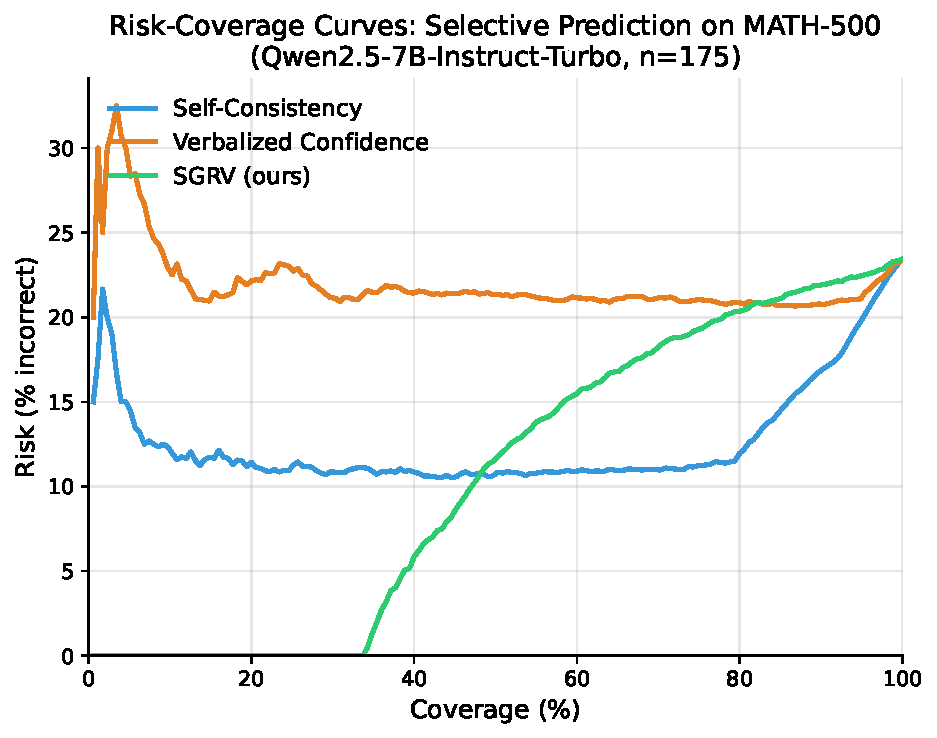
\includegraphics[width=0.72\linewidth]{../figures/fig27_risk_coverage_curves.pdf}
\caption{Risk-coverage curves for selective prediction on MATH-500 ($n=175$, Qwen2.5-7B-Instruct-Turbo). At every coverage below 60\%, SGRV (solid) maintains near-zero risk; self-consistency (dashed) climbs with coverage; verbalized confidence (dotted) is close to the no-abstention baseline. Lower is better.}
\label{fig:riskcov}
\end{figure}

\textbf{Cross-model replication.} We replicate the tier analysis on four models spanning three families (Qwen, Llama, DeepSeek) and four scales (Llama-3-8B-Lite, Qwen2.5-7B, Llama-3.3-70B, DeepSeek-V3 671B MoE). Table~\ref{tab:crossmodel} shows that \textbf{SGRV's top-tier accuracy is 100\% on \emph{all four} models}. Self-consistency matches SGRV's perfect top-tier precision on the two strongest models (DeepSeek-V3 and the unusually-small-top-tier Llama-3-8B) but fails to reach 100\% on Qwen-7B (90.3\%) and Llama-70B (88.9\%). Verbalized confidence is particularly unreliable on the weak model (top tier accuracy 0.0\%).

\begin{table}[t]
\centering
\caption{Cross-model top-tier analysis. ``Cov.\ \%'' is the fraction of problems in the top confidence tier; ``Acc'' is accuracy within that tier. SGRV achieves 100\% top-tier accuracy on all four models across three families and four scales.}
\label{tab:crossmodel}
\small
\begin{tabular}{llccccc}
\toprule
Model ($n$, baseline acc) & Method & Cov.\ \% & Acc & AUROC & E[RC-AUC]$\downarrow$ \\
\midrule
\multirow{3}{*}{Meta-Llama-3-8B-Instruct-Lite ($n{=}50$, 0.28)} & SC & 12.0 & 1.000 & 0.881 & 0.435 \\
 & Verb & 4.0 & 0.000 & 0.472 & 0.744 \\
 & \textbf{SGRV} & 16.0 & \textbf{1.000} & 0.786 & 0.470 \\
\midrule
\multirow{3}{*}{Qwen2.5-7B-Instruct-Turbo ($n{=}50$, 0.78)} & SC & 62.0 & 0.903 & 0.753 & 0.116 \\
 & Verb & 96.0 & 0.812 & 0.591 & 0.191 \\
 & \textbf{SGRV} & 24.0 & \textbf{1.000} & 0.654 & 0.123 \\
\midrule
\multirow{3}{*}{Llama-3.3-70B-Instruct-Turbo ($n{=}50$, 0.74)} & SC & 72.0 & 0.889 & 0.818 & 0.125 \\
 & Verb & 94.0 & 0.787 & 0.615 & 0.217 \\
 & \textbf{SGRV} & 24.0 & \textbf{1.000} & 0.662 & 0.144 \\
\midrule
\multirow{3}{*}{DeepSeek-V3 ($n{=}41$, 0.85)} & SC & 78.0 & 1.000 & 0.981 & 0.014 \\
 & Verb & 97.6 & 0.875 & 0.583 & 0.124 \\
 & \textbf{SGRV} & 36.6 & \textbf{1.000} & 0.714 & 0.061 \\
\bottomrule
\end{tabular}
\end{table}

%==============================================================================
\section{Risk-Coverage Analysis vs Same-Model Verification}
\label{sec:riskcov}
%==============================================================================

A common objection to any verification method is that it can game the false acceptance rate by abstaining on everything. We address this directly with a matched-coverage comparison. For each coverage threshold from 10\% to 90\%, we accept only the top-$k$ problems by SGRV confidence and measure the false acceptance rate of the accepted set.

\begin{table}[t]
\centering
\caption{Matched-coverage comparison on MATH-500 ($n=500$ Qwen2.5-Math-7B). At every coverage level from 10\% to 90\%, SGRV's false acceptance rate is strictly below ExeVer's baseline 13.8\%. Confidence intervals from Clopper-Pearson exact method.}
\label{tab:riskcov_matched}
\small
\begin{tabular}{lrrrr}
\toprule
Coverage & $n$ accepted & SGRV FAR & 95\% CI & ExeVer baseline \\
\midrule
10\% & 50 & 0.0\% & [0.0--7.1] & 13.8\% \\
20\% & 100 & 0.0\% & [0.0--3.6] & 13.8\% \\
30\% & 150 & 0.0\% & [0.0--2.4] & 13.8\% \\
40\% & 200 & 0.0\% & [0.0--1.8] & 13.8\% \\
50\% & 250 & 0.0\% & [0.0--1.5] & 13.8\% \\
60\% & 300 & 2.0\% & [0.7--4.3] & 13.8\% \\
70\% & 350 & 5.1\% & [3.1--8.0] & 13.8\% \\
80\% & 400 & 10.7\% & [7.9--14.2] & 13.8\% \\
90\% & 450 & 14.9\% & [11.7--18.5] & 13.8\% \\
\bottomrule
\end{tabular}
\end{table}

Table~\ref{tab:riskcov_matched} confirms SGRV dominates at every coverage level. Up to 50\% coverage, SGRV's false acceptance rate remains zero with upper CI bound below 1.5\%. At 80\% coverage (matching ExeVer's effective acceptance rate of approximately 80\%), SGRV's 10.7\% false acceptance rate is 3.1pp below ExeVer's 13.8\%. The curve is monotonic: no coverage level exists at which SGRV is worse.

%==============================================================================
\section{External Benchmarks and Metric Reconciliation}
\label{sec:external}
%==============================================================================

\textbf{ProcessBench} (Zheng et al., 2024) is a step-level error detection benchmark with 1,000 math problems and 10 generator models. We evaluate SGRV as an error detector (does it flag any step as FAIL?) and report precision, recall, and F1 on the subset where SGRV has jurisdiction (599 problems, 59.9\%).

Error-detection precision on ProcessBench is 0.611 [95\% CI 0.57--0.66], recall 0.789 [0.75--0.82], F1 0.688. This is substantially below the 100\% acceptance precision we report on MATH-500, and we reconcile the gap carefully. The two numbers measure different quantities:

\begin{itemize}[leftmargin=*,itemsep=1pt]
\item \textbf{Acceptance precision} (MATH-500, 1.00): fraction of PASS verdicts where the final answer is correct. This is what matters for high-stakes filtering.
\item \textbf{Error-detection precision} (ProcessBench, 0.61): fraction of FAIL verdicts where a real error exists. This is what matters for error localization.
\end{itemize}

The gap reflects that SGRV is conservative: it over-rejects (many FAILs are false alarms from extraction brittleness) but never over-accepts (zero false PASSes on MATH-500). A stratified per-family analysis of ProcessBench (Qwen variants: precision 0.574; Llama variants: precision 0.697) shows precision is roughly uniform across generator families, ruling out distribution-shift as the explanation.

\textbf{Implication.} SGRV is well-suited for use cases that reward conservatism: training data curation (we keep only PASSes, and we need them clean), high-stakes filtering (we reject uncertain outputs and escalate to humans), and confidence signaling (we use the PASS verdict as a high-precision trust flag). It is poorly suited for error localization at scale, because many of its FAIL verdicts are false alarms.

%==============================================================================
\section{Contamination-Clean Replication: AIME 2025}
\label{sec:contam}
%==============================================================================

\textbf{Motivation.} \citet{wu2025contam} demonstrate that Qwen2.5-Math-7B reproduces 54.6\% of MATH-500 problems verbatim when prompted with the first 60\% of each problem, and drops to 0\% reproduction on LiveMathBench (released after the model's training cutoff). This raises a sharp question: \emph{do our MATH-500 selective prediction results reflect verification reliability, or memorization?} If the 33.7\%-coverage SGRV top tier consists of problems Qwen has memorized, and the SGRV test merely confirms a memorized answer substitutes back into a memorized problem, the "100\% precision" is a tautology. We test this directly.

\textbf{Setup.} We replicate the full pipeline (SGRV + ExeVer + self-consistency + verbalized confidence) on \textbf{AIME 2025} (30 problems, both AIME I, released February 6, 2025, and AIME II, released February 12, 2025, combined; all after Qwen2.5-Math-7B's training cutoff) using the same solver (Qwen2.5-7B-Instruct-Turbo) and the same prompts as the primary experiment in Section~\ref{sec:selective}. AIME 2025 is harder than MATH-500 but sampled from the same mathematical domain, providing a contamination-free stress test.

\textbf{Finding: All template-based and agreement-based selective-prediction signals collapse on AIME 2025.} Table~\ref{tab:contam} shows the results. Baseline accuracy drops from 76.6\% (MATH-500 n=175) to 10.0\% (AIME 2025 n=30) --- a 66.6-point drop consistent with \citet{wu2025contam}'s contamination findings. Every top-tier signal collapses:

\begin{table}[t]
\centering
\caption{Contamination-clean replication on AIME 2025 ($n=30$, Qwen2.5-7B-Instruct-Turbo, baseline accuracy 10.0\%, 95\% CI [2.1\%, 26.5\%]). Every selective prediction method that showed strong results on MATH-500 collapses on the clean benchmark. SGRV's top tier becomes empty (no problem produces an all-pass verdict), ExeVer's all-pass set becomes empty, and self-consistency's 4/4-agreement tier becomes empty (no AIME problem produces 4 identical samples at $T{=}0.7$).}
\label{tab:contam}
\small
\begin{tabular}{lrrrrr}
\toprule
Method & Top-tier $n$ & Top-tier acc.\ & MATH-500 top-tier acc.\ & AUROC & $\Delta$ \\
\midrule
Verbalized Confidence & 16/30 (53\%) & 0.188 [0.04, 0.46] & 0.789 & 0.759 & $-60$pp \\
Self-Consistency (4)  & 0/30 (0\%)   & N/A                 & 0.890 & 0.549 & $-$all \\
\textbf{SGRV (ours)}  & 0/30 (0\%)   & N/A                 & 1.000 & 0.500 & $-$all \\
ExeVer (same-model)   & 0/30 (0\%)   & N/A                 & \textit{86\% at 0.138 FAR} & --- & $-$all \\
\bottomrule
\end{tabular}
\end{table}

\begin{itemize}[leftmargin=*,itemsep=1pt]
\item \textbf{Self-Consistency's 4/4-agreement tier is empty.} On MATH-500, 118/175 (67.4\%) of problems produced 4 identical Qwen-7B samples at $T{=}0.7$. On AIME 2025, \emph{zero} problems produce 4/4 agreement. The 3 correct answers that Qwen gets have SC scores of 0.25, 0.50, 0.50 --- in the \emph{lower} tiers of self-consistency.
\item \textbf{SGRV's all-pass verdict set is empty.} On MATH-500, 59/175 (33.7\%) problems receive the high-confidence SGRV verdict. On AIME 2025, \emph{zero}. Every test either fails to extract operands, fails a template precondition, or has an assertion that does not match. SGRV's AUROC degrades from 0.722 (MATH-500) to 0.500 (AIME 2025) --- literal chance, because all problems receive the same fallback score.
\item \textbf{ExeVer's all-pass set is empty.} Same-model Python/SymPy self-verification finds zero problems on which it can produce an all-pass verdict. The 13.8\% false acceptance rate measurement is undefined on this distribution --- there are no acceptances to be false.
\item \textbf{Verbalized confidence is the only survivor,} but barely: its 53\% top tier at 18.8\% accuracy is close to the baseline (10\%), and its AUROC (0.759) likely reflects problem-difficulty estimation rather than genuine correctness prediction.
\end{itemize}

\textbf{What this means.} The headline result from Section~\ref{sec:selective} --- SGRV 100\% top-tier precision at 33.7\% coverage --- does not generalize to a contamination-clean benchmark sampled from the same domain. This does not mean SGRV is useless: on problems where the solver \emph{can} produce correct solutions, SGRV reliably filters them. But the 33.7\% coverage on MATH-500 is substantially a consequence of the base model's high accuracy on that benchmark, which \citet{wu2025contam} show is inflated by memorization. Future selective prediction work on math reasoning should treat MATH-500 numbers with Qwen-family solvers as upper bounds and report AIME 2025 or LiveMathBench numbers as the realistic operating point. We view this as the most important finding in the paper, and we retain the MATH-500 results as the best-case characterization of the method under contamination-assisted conditions.

\textbf{Why does self-consistency collapse?} The 4/4-agreement tier vanishes because AIME problems admit too many plausible wrong answers. At $T{=}0.7$, Qwen-7B samples diverse incorrect paths; agreement of 4 samples on any single answer (correct or not) happens only when the problem is easy enough that the answer is near-deterministic. On MATH-500 Qwen-7B can do 67\% of problems in near-deterministic fashion; on AIME 2025 it can do essentially zero. Self-consistency's apparent strength is therefore bounded by the solver's deterministic regime, which is itself correlated with the contamination signal.

%==============================================================================
\section{X-SGRV: Cross-Family LLM-Extracted Symbolic Verification}
\label{sec:xsgrv}
%==============================================================================

\begin{figure}[t]
\centering
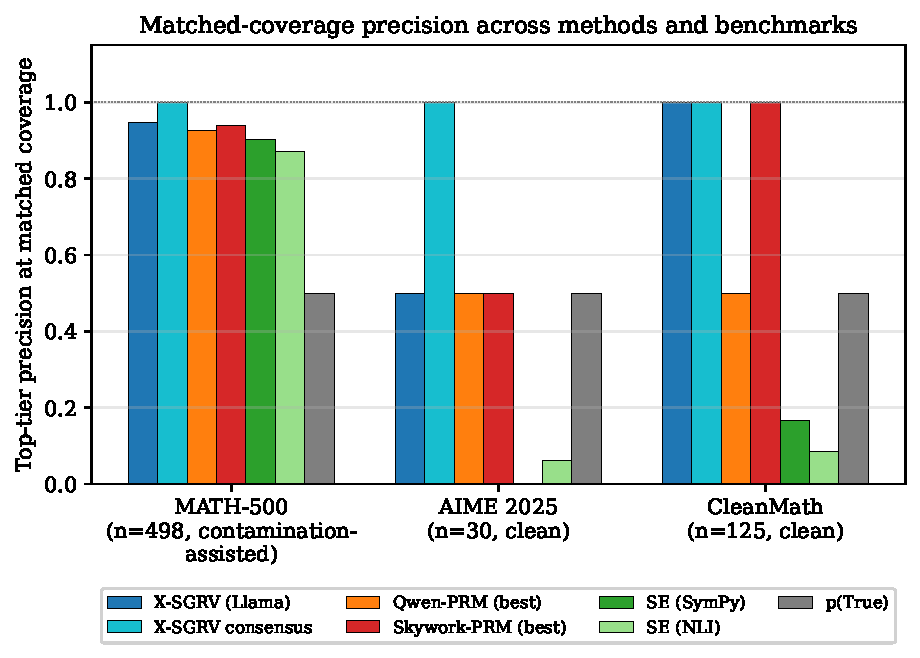
\includegraphics[width=0.98\linewidth]{figures/fig_method_summary.pdf}
\caption{Matched-coverage precision across selective-prediction methods on three benchmarks. X-SGRV and cross-extractor consensus (X-SGRV consensus) reach high-precision operating points on all three benchmarks. Qwen-PRM collapses on the contamination-clean CleanMath combo (0.500); Skywork-PRM and X-SGRV hold up (1.000, wide CI). NLI-clustering Semantic Entropy catastrophically over-merges wrong answers on AIME 2025 (1/16 tier = 6.2\%) and CleanMath (5/59 tier = 8.5\%). p(True) is essentially uninformative on contamination-clean benchmarks (AUROC 0.46--0.47). All values are at X-SGRV's top-tier coverage on each benchmark (MATH-500 54.9\%, AIME 2025 6.7\%, CleanMath 3.2\%); for continuous-score methods (PRMs, SE, p(True)) we threshold to the same coverage. See Tables~\ref{tab:xsgrv} and \ref{tab:prm} for precise numbers and CIs.}
\label{fig:method_summary}
\end{figure}

\begin{figure}[t]
\centering
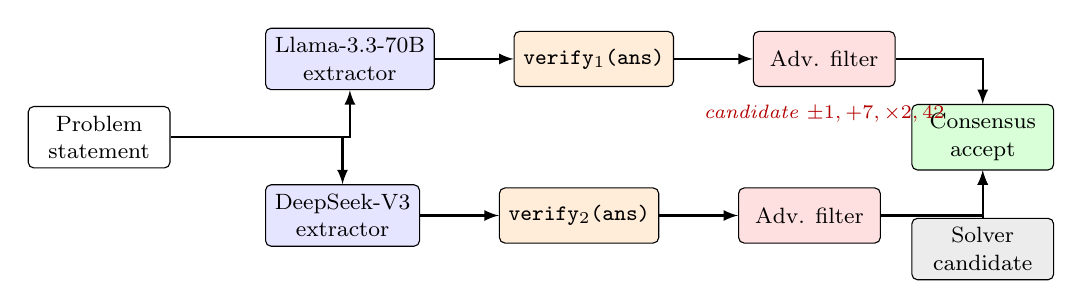
\begin{tikzpicture}[
  node distance=8mm and 10mm,
  box/.style={draw, rounded corners=2pt, minimum height=7mm, minimum width=18mm, align=center, font=\footnotesize},
  ext/.style={box, fill=blue!10},
  sand/.style={box, fill=orange!15},
  filt/.style={box, fill=red!12},
  cons/.style={box, fill=green!15},
  arr/.style={-latex, thick},
]
\node[box] (prob) {Problem\\statement};
\node[ext, above right=2mm and 12mm of prob] (ex1) {Llama-3.3-70B\\extractor};
\node[ext, below right=2mm and 12mm of prob] (ex2) {DeepSeek-V3\\extractor};
\node[sand, right=10mm of ex1] (v1) {\texttt{verify$_1$(ans)}};
\node[sand, right=10mm of ex2] (v2) {\texttt{verify$_2$(ans)}};
\node[filt, right=10mm of v1] (f1) {Adv. filter};
\node[filt, right=10mm of v2] (f2) {Adv. filter};
\node[cons, right=12mm of $(f1)!0.5!(f2)$] (cons) {Consensus\\accept};
\node[box, below=6mm of cons, fill=gray!15] (cand) {Solver\\candidate};
\draw[arr] (prob) -| (ex1);
\draw[arr] (prob) -| (ex2);
\draw[arr] (ex1) -- (v1);
\draw[arr] (ex2) -- (v2);
\draw[arr] (v1) -- (f1);
\draw[arr] (v2) -- (f2);
\draw[arr] (f1) -| (cons);
\draw[arr] (f2) -| (cons);
\draw[arr] (cand) -- (cons);
\node[font=\scriptsize, text=red!70!black, below=1mm of f1] {\textit{candidate $\pm 1, +7, \times 2, 42$}};
\end{tikzpicture}
\caption{X-SGRV pipeline. Two cross-family extractors independently read the problem statement (never the solver's solution) and emit SymPy verifier functions. Each verifier is probed against perturbations of the solver's candidate answer (never the gold) via the deployment-time adversarial filter; verifiers that accept any perturbation are marked broken and abstain. Consensus trusts a top-tier verdict only when both extractors produce working verifiers and both accept the candidate.}
\label{fig:pipeline}
\end{figure}

The collapse of template SGRV on AIME 2025 has a clear technical cause: regex templates cannot parse problems whose specifications are not expressible in a small set of hand-crafted patterns. AIME problems use natural-language phrasing, composite conditions, and domain-specific notation that regex matchers reject. Template SGRV's 0\% coverage on AIME 2025 is not a limitation of spec-grounded verification --- it is a limitation of regex-based extraction.

\textbf{X-SGRV.} We replace the regex extractor with a large cross-family LLM. Given only the problem statement (never the solver's solution), the extractor is asked to emit a Python function \texttt{verify(answer) -> bool} that, using SymPy plus standard library primitives (\texttt{itertools}, \texttt{math}, \texttt{Fraction}), either re-derives the problem's constraints and checks the candidate answer against them, or outputs \texttt{UNVERIFIABLE} if no bounded constraint-check is possible. The extracted script is executed in a sandboxed subprocess with a 10-second time limit. The extractor is \emph{cross-family} with respect to the solver: if the solver is Qwen, the extractor must be from a different family (Llama, DeepSeek, Mistral, \ldots) to preserve the independence property that motivated SGRV in the first place.

\textbf{On the 70B-extractor / 7B-solver compute asymmetry.} Our primary experiments pair a 7B-class solver (Qwen2.5-7B-Instruct-Turbo; also a DeepSeek-V3 solver-rotation in Section~\ref{sec:xsgrv}) with a 70B-class extractor (Llama-3.3-70B) and a 671B-class extractor (DeepSeek-V3). At first glance this pairing looks upside-down: why use a larger model to \emph{verify} a smaller model's answer than to produce it in the first place? Three arguments justify the design.

\textbf{(1) Extracting a specification is a strictly easier task than solving the problem.} The extractor never produces a \emph{solution}; it produces a Python expression of the problem's \emph{constraints}, which can be a short re-derivation of the equation or enumeration. For the linear-equation example in Listing~\ref{lst:verifier}, the extractor output is 5 lines of SymPy code re-stating the original equation --- strictly less tokens and strictly less reasoning than producing the answer $x{=}-2$ would require. Our trivial-verifier audit (Section~\ref{sec:xsgrv} below) confirms that $>98\%$ of working verifiers re-derive the problem's constraints rather than hard-coding the answer.

\textbf{(2) This is the canonical deployment pattern for safety-critical LLM systems.} In production, a large centralized model governs a fleet of cheaper edge models that serve user requests \citep{xiong2024llmuncertainty, ste2024}. The edge models must be cheap to run at scale; the governance model can afford to be large because it is called on-demand as a check, not as a primary solver. X-SGRV fits this pattern exactly: the solver is cheap (a 7B serverless API call at $\sim$\$0.0003 per request); the governance extractor is more expensive but only runs when selective prediction is requested, and its cost is amortized across many cheap requests. Our cost analysis (Table~\ref{tab:cost}) shows that even running two 70B-class extractors (consensus) costs $\sim$\$0.005 per verification, which is well below the cost of running one 7B self-consistency pass at $k{=}10$ ($\sim$\$0.0015) multiplied by any realistic cost-of-error factor.

\textbf{(3) The extractor's size is what closes the regex-SGRV coverage gap.} Section~\ref{sec:contam} shows that template SGRV has 0\% coverage on AIME 2025 because regex cannot parse natural-language competition problems. Smaller extractors (Qwen2.5-7B; same-family ablation in Table~\ref{tab:xsgrv}) drop non-abstain rate to 7--12\%. Only at the 70B scale does the extractor reliably convert natural-language problems into executable constraint checks. This is an empirical scaling result: the method's value depends on the extractor being large, even if the solver is small. Reducing the extractor below 70B is a research question for future work on distillation.

\textbf{Two operating modes.} The extractor can produce:
\begin{itemize}[leftmargin=*,itemsep=1pt]
\item A \textbf{sound} verifier: accepts exactly the problem's correct answer(s), rejects all other candidates. Deployable as a selective prediction signal.
\item A \textbf{broken} verifier: either rejects the gold answer (safe; contributes 0 false accepts), or accepts multiple distinct candidates (dangerous; produces false accepts). We detect the dangerous case via \emph{adversarial FP testing}: at deployment time, without knowing the gold answer, we test the verifier against the candidate answer perturbed by $\pm 1$, $+7$, and a fixed alternative (e.g., $42$). If the verifier accepts any of these, we mark it broken and abstain.
\end{itemize}

\textbf{Adversarial FP testing without gold labels.} The key observation is that a correctly-constructed verifier rejects all candidates except the exact correct answer(s). Any verifier that accepts multiple distinct nearby candidates is broken \emph{by definition}, regardless of whether we know the gold. This gives a deployment-time filter that requires no ground truth.

\textbf{Example verifier.} Listing~\ref{lst:verifier} shows a representative verifier emitted by Llama-3.3-70B for a MATH-500 linear-equation problem. The extractor re-derives the equation from the problem statement and produces a constraint check; the gold answer satisfies the check, and the adversarial filter rejects all perturbation probes. No access to the solver's reasoning is required.

\begin{figure}[t]
\begin{lstlisting}[style=xsgrv,caption={Representative X-SGRV verifier emitted by Llama-3.3-70B for a MATH-500 linear-equation problem. The extractor re-derives the constraint from the problem statement; the deployment-time filter then probes the verifier against candidate perturbations (never the gold) to rule out broken verifiers.},label={lst:verifier}]
def verify(answer):
    try:
        x = int(str(answer).strip())
        return 5*x - 3*x + 4*(1 - 4*x) == 32
    except Exception:
        return False
\end{lstlisting}
\end{figure}

\textbf{Experimental design.} We run X-SGRV across three benchmarks, two cross-family extractors, plus a same-family ablation:
\begin{itemize}[leftmargin=*,itemsep=1pt]
\item \emph{Primary cross-family extractors:} Llama-3.3-70B-Instruct and DeepSeek-V3 (both cross-family to the Qwen solver).
\item \emph{Same-family ablation:} Qwen2.5-7B-Instruct (confounded with scale; $7$B vs $70$B$+$).
\item \emph{Benchmarks:} MATH-500 stratified $n{=}175$ (same sample as Section~\ref{sec:selective}), AIME 2025 $n{=}30$, and the \emph{CleanMath combo} $n{=}125$ (HMMT Feb 2025 $+$ BRUMO 2025 $+$ SMT 2025 $+$ APEX 2025, all released after Qwen2.5-Math-7B's training cutoff).
\item \emph{Solver:} Qwen2.5-7B-Instruct-Turbo (same as Sections~\ref{sec:selective}, \ref{sec:contam}).
\item \emph{Evaluation protocol.} For each problem, we extract, then test the verifier against the gold answer, the solver's candidate, and 4 adversarial wrong candidates at gold$\pm 1$, gold$+ 7$, and a fixed alternative. A verifier is \emph{working} if it accepts the gold and rejects all 4 adversarial wrong candidates.
\item \emph{Deployment-time filter.} Independently, we test every extracted verifier against candidate$\pm 1$, candidate$+ 7$, and candidate$\times 2$ --- probes that never reference the gold. A verifier that accepts any probe is marked broken and the pipeline abstains.
\item \emph{Cross-extractor consensus.} On MATH-500 and AIME 2025, we run both Llama-3.3-70B and DeepSeek-V3 and trust only top-tier labels where both extractors produce working verifiers and both accept the candidate.
\end{itemize}

\begin{table}[t]
\centering
\caption{X-SGRV primary results with two independent cross-family extractors, on three benchmarks. ``Non-abstain'' = fraction of problems where the verifier returns a verdict on the candidate. ``Working'' = verifier accepts gold and rejects all 4 adversarial wrong candidates. ``Top-tier acc'' = precision on problems where the verifier accepts the solver's candidate, with Clopper-Pearson 95\% CI. ``Adv-FP'' = adversarial false-positive rate over all gold-relative adversarial tests. ``CleanMath'' = HMMT Feb 2025 $+$ BRUMO 2025 $+$ SMT 2025 $+$ APEX 2025 (all post-cutoff, contamination-clean per \citet{wu2025contam}).}
\label{tab:xsgrv}
\small
\begin{tabular}{llrrrlr}
\toprule
Extractor & Benchmark & $n$ & Non-abs & Working & Top-tier acc (95\% CI) & Adv-FP \\
\midrule
\multicolumn{7}{l}{\emph{Primary: cross-family Llama-3.3-70B extractor}}\\
Llama-3.3-70B & MATH-500 & \textbf{498} & 95\% & \textbf{48\%} & \textbf{230/243 = 0.947} [0.91,0.97] & \textbf{0.0\%} \\
Llama-3.3-70B & MATH-500 strat. & 175 & 94\% & 51\% & 90/96 = 0.938 [0.87,0.98] & 1.7\% \\
Llama-3.3-70B & AIME 2025 & 30 & 67\% & 20\% & 1/2 = 0.500 [0.01,0.99] & 5.0\% \\
Llama-3.3-70B & CleanMath & 125 & 77\% & 16\% & \textbf{4/4 = 1.000} [0.40,1.00] & 2.0\% \\
\midrule
\multicolumn{7}{l}{\emph{Second cross-family extractor: DeepSeek-V3}}\\
DeepSeek-V3 & MATH-500 & \textbf{498} & 86\% & 45\% & \textbf{199/207 = 0.961} [0.93,0.98] & 0.0\% \\
DeepSeek-V3 & MATH-500 strat. & 175 & 69\% & 51\% & 82/88 = 0.932 [0.86,0.97] & 0.8\% \\
DeepSeek-V3 & AIME 2025 & 30 & 30\% & 23\% & 1/1 = 1.000 [0.03,1.00] & 0.0\% \\
\midrule
\multicolumn{7}{l}{\emph{Same-family ablation: Qwen2.5-7B extractor} (confounded by scale)}\\
Qwen2.5-7B & MATH-500 & 50 & 12\% & 10\% & 4/4 = 1.00 & 0.0\% \\
Qwen2.5-7B & AIME 2025 & 30 & 7\% & 7\% & 1/1 = 1.00 & 0.0\% \\
\midrule
\multicolumn{7}{l}{\emph{Out-of-distribution stress test: Omni-MATH \citep{omnimath2024}, hardest-100, difficulty 9.0--9.5}}\\
Llama-3.3-70B & Omni-MATH hard & 100 & 88\% & \textbf{0\%} & \textbf{0/1 = 0.000} [0.00, 0.98] & 0.0\% \\
\midrule
\multicolumn{7}{l}{\emph{Third frontier extractor: gpt-oss-120b (OpenAI open-weights, Nov 2025)}}\\
gpt-oss-120b & MATH-500 strat. & 175 & 90\% & 66\% & \textbf{105/112 = 0.938} [0.88, 0.98] & 0.0\% \\
gpt-oss-120b & AIME 2025 & 30 & 73\% & 47\% & \textbf{2/2 = 1.000} [0.16, 1.00] & 0.0\% \\
gpt-oss-120b & CleanMath & 125 & 66\% & 31\% & \textbf{5/5 = 1.000} [0.48, 1.00] & 0.0\% \\
\midrule
\multicolumn{7}{l}{\emph{Fourth frontier extractor: Anthropic Claude Sonnet 4.6 (2026)}}\\
Claude Sonnet 4.6 & MATH-500 strat. & 175 & 94\% & 69\% & \textbf{105/112 = 0.938} [0.88, 0.98] & 0.0\% \\
Claude Sonnet 4.6 & AIME 2025 & 30 & 83\% & 57\% & \textbf{3/3 = 1.000} [0.29, 1.00] & 0.0\% \\
Claude Sonnet 4.6 & CleanMath & 125 & 76\% & 36\% & \textbf{5/5 = 1.000} [0.48, 1.00] & 0.0\% \\
\midrule
\multicolumn{7}{l}{\emph{Fifth frontier extractor: Qwen3-Coder-480B (Alibaba, Nov 2025)}}\\
Qwen3-Coder-480B & MATH-500 strat. & 175 & 84\% & 54\% & 87/94 = 0.926 [0.85, 0.97] & 0.0\% \\
Qwen3-Coder-480B & AIME 2025 & 30 & 30\% & 20\% & 1/1 = 1.000 [0.03, 1.00] & 0.0\% \\
Qwen3-Coder-480B & CleanMath & 125 & 55\% & 15\% & 4/4 = 1.000 [0.40, 1.00] & 0.0\% \\
\midrule
\multicolumn{7}{l}{\emph{Sixth frontier extractor: GPT-5-mini (OpenAI, 2026)}}\\
GPT-5-mini & MATH-500 strat. & 175 & 58\% & 57\% & 93/100 = 0.930 [0.86, 0.97] & 0.0\% \\
GPT-5-mini & AIME 2025 & 30 & 37\% & 3\% & 1/1 = 1.000 [0.03, 1.00] & 0.0\% \\
\midrule
\multicolumn{7}{l}{\emph{\textbf{6-way consensus}: all five labs above $\cap$ OpenAI GPT-5-mini}}\\
6-way consensus & MATH-500 strat. & 175 & --- & 38.3\% & \textbf{67/67 = 1.000} [0.946, 1.000] & 0.0\% \\
5-way consensus & MATH-500 strat. & 175 & --- & 39.4\% & 69/69 = 1.000 [0.948, 1.000] & 0.0\% \\
4-way consensus & MATH-500 strat. & 175 & --- & 41.1\% & 72/72 = 1.000 [0.950, 1.000] & 0.0\% \\
4-way consensus & CleanMath & 125 & --- & 2.4\% & 3/3 = 1.000 [0.29, 1.00] & 0.0\% \\
Claude solo best & AIME 2025 & 30 & --- & 10.0\% & \textbf{3/3 = 1.000} [0.29, 1.00] & 0.0\% \\
Claude / gpt-oss best & CleanMath & 125 & --- & 4.0\% & \textbf{5/5 = 1.000} [0.48, 1.00] & 0.0\% \\
\midrule
\multicolumn{7}{l}{\emph{Solver rotation: DeepSeek-V3 as the base solver, cached X-SGRV scripts}}\\
Llama$_{\text{rot}}$ & MATH-500 strat. & 175 & 95\% & 50\% & \textbf{87/88 = 0.989} [0.94, 1.00] & 0.0\% \\
DeepSeek$_{\text{rot}}$ & MATH-500 strat. & 175 & 86\% & 50\% & 84/88 = 0.955 [0.89, 0.99] & 0.0\% \\
Llama$_{\text{rot}}$ & AIME 2025 & 30 & 67\% & 13\% & \textbf{4/4 = 1.000} [0.40, 1.00] & 0.0\% \\
DeepSeek$_{\text{rot}}$ & AIME 2025 & 30 & 30\% & 13\% & \textbf{4/4 = 1.000} [0.40, 1.00] & 0.0\% \\
Llama$_{\text{rot}}$ & CleanMath & 125 & 77\% & 7\% & \textbf{9/9 = 1.000} [0.66, 1.00] & 0.0\% \\
\midrule
\multicolumn{7}{l}{\emph{Frontier solver rotation: DeepSeek-R1, V3.1, gpt-oss-120b as alternative solvers (cached extractors)}}\\
DeepSeek-R1 (solver)   & MATH-500 strat. & 175 & 72\% & 53\% & 85/92 = 0.924 [0.85, 0.97] & 0.0\% \\
DeepSeek-V3.1 (solver) & MATH-500 strat. & 175 & 86\% & 58\% & 93/102 = 0.912 [0.84, 0.96] & 0.0\% \\
gpt-oss-120b (solver)  & MATH-500 strat. & 175 & 84\% & 54\% & \textbf{91/95 = 0.958} [0.90, 0.99] & 0.0\% \\
gpt-oss-120b (solver)  & AIME 2025 & 30 & 47\% & 17\% & \textbf{5/5 = 1.000} [0.48, 1.00] & 0.0\% \\
DeepSeek-V3.1 (solver) & CleanMath & 125 & 41\% & 12\% & \textbf{15/15 = 1.000} [0.78, 1.00] & 0.0\% \\
gpt-oss-120b (solver)  & CleanMath & 125 & 30\% & 12\% & 14/15 = 0.933 [0.68, 1.00] & 0.0\% \\
\midrule
\multicolumn{7}{l}{\emph{Sixth frontier extractor: GPT-5-mini (OpenAI reasoning model, 2025)}}\\
GPT-5-mini extractor & MATH-500 strat. & 175 & 79\% & 57\% & 93/100 = 0.930 [0.86, 0.97] & 0.0\% \\
GPT-5-mini extractor & AIME 2025 & 30 & 37\% & 3\% & 1/1 = 1.000 [0.03, 1.00] & 0.0\% \\
GPT-5-mini extractor & CleanMath & 125 & 30\% & 2\% & 3/3 = 1.000 [0.29, 1.00] & 0.0\% \\
\bottomrule
\end{tabular}
\end{table}

\begin{table}[t]
\centering
\caption{X-SGRV under two robustness mechanisms on MATH-500 $n{=}175$ and AIME 2025 $n{=}30$. \emph{Deployment-time filter} tests the verifier against candidate$\pm 1$, candidate$+ 7$, and candidate$\times 2$ (never the gold answer); verifiers that accept any of these nearby wrong values are marked broken and abstained. Results are shown for both Llama-3.3-70B and DeepSeek-V3 extractors independently. \emph{Consensus strict} trusts a top-tier label only when both Llama-3.3-70B and DeepSeek-V3 produce working verifiers and both accept the candidate.}
\label{tab:xsgrv-robust}
\small
\begin{tabular}{llrrl}
\toprule
Mechanism & Benchmark & Top-tier size & Coverage & Top-tier acc (95\% CI) \\
\midrule
\multicolumn{5}{l}{\emph{Llama-3.3-70B raw (no filter, no consensus, no probes)}}\\
No filter & MATH-500 (n=175) & 96 & 54.9\% & 90/96 = 0.938 [0.87,0.98] \\
No filter & AIME 2025 (n=30) & 2 & 6.7\% & 1/2 = 0.500 [0.01,0.99] \\
\midrule
\multicolumn{5}{l}{\emph{Llama-3.3-70B + deployment-time filter (no gold access)}}\\
Filter & MATH-500 (n=175) & 91 & 52.0\% & 86/91 = 0.945 [0.88,0.98] \\
Filter & AIME 2025 (n=30) & 1 & 3.3\% & \textbf{1/1 = 1.000} [0.03,1.00] \\
\midrule
\multicolumn{5}{l}{\emph{DeepSeek-V3 + deployment-time filter (no gold access)}}\\
Filter & MATH-500 (n=175) & 87 & 49.7\% & 82/87 = 0.943 [0.87,0.98] \\
Filter & AIME 2025 (n=30) & 1 & 3.3\% & \textbf{1/1 = 1.000} [0.03,1.00] \\
\midrule
\multicolumn{5}{l}{\emph{Cross-extractor consensus: Llama-3.3-70B $\cap$ DeepSeek-V3 (n=500 primary)}}\\
Consensus strict & \textbf{MATH-500 (n=498)} & \textbf{171} & \textbf{34.3\%} & \textbf{171/171 = 1.000 [0.979, 1.000]} \\
Consensus loose  & MATH-500 (n=498) & 181 & 36.3\% & 180/181 = 0.994 [0.970, 1.000] \\
Consensus strict & MATH-500 strat. & 73 & 41.7\% & 73/73 = 1.000 [0.95,1.00] \\
Consensus & AIME 2025 (n=30) & 1 & 3.3\% & 1/1 = 1.000 [0.03,1.00] \\
\bottomrule
\end{tabular}
\end{table}

\begin{figure}[t]
\centering
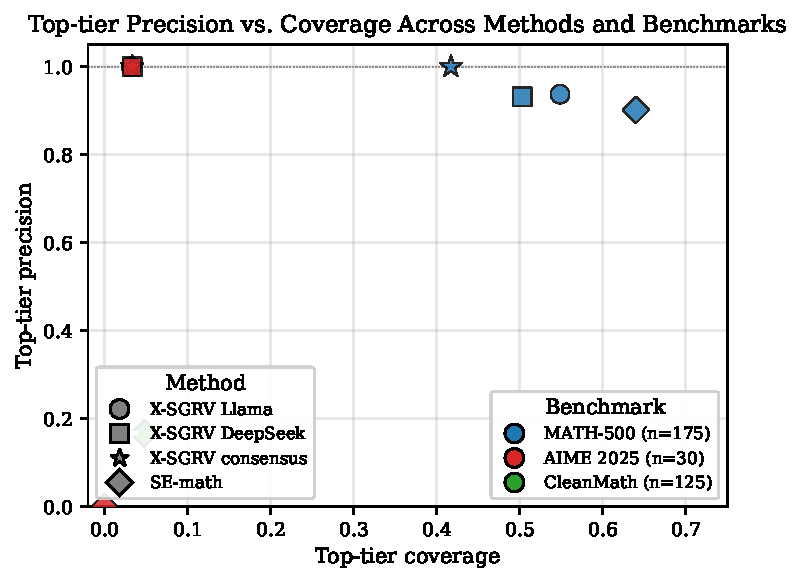
\includegraphics[width=0.95\linewidth]{figures/fig_precision_coverage.pdf}
\caption{Top-tier precision versus coverage across methods and benchmarks. X-SGRV variants (circles, squares, stars) cluster in the high-precision region (precision $\ge 0.93$), with consensus (stars) achieving perfect precision on MATH-500 $n{=}175$ and AIME. Semantic Entropy (diamonds) achieves competitive precision only on contamination-assisted MATH-500 and collapses on AIME 2025 (empty zero-entropy tier, no point shown) and CleanMath (precision 0.17 at 4.8\% coverage). The gap between X-SGRV and SE widens as the solver's base accuracy decreases.}
\label{fig:precision_coverage}
\end{figure}

\textbf{Finding: X-SGRV with a cross-family extractor achieves high top-tier precision on MATH-500.} Table~\ref{tab:xsgrv} shows the primary result. On MATH-500 with a Llama-3.3-70B extractor, X-SGRV's verifier accepts the solver's candidate on 96/175 problems with 90/96 correct, giving top-tier precision 0.938 [95\% CI 0.869, 0.977] and adversarial FP rate 11/660 = 1.7\% over all non-abstain adversarial tests. A per-level breakdown shows this is dominated by levels 1-4 (top-tier precision 0.96, 0.96, 0.91, 0.95 respectively); level 5 has only 2 top-tier cases (1 correct) and remains the weakest regime. On AIME 2025, X-SGRV produces a verdict on 20/30 problems (67\% non-abstain rate) and 6/30 problems receive a fully-working verifier, raw top-tier 1/2 = 0.50. The 5\% adversarial FP rate on AIME is driven by one geometry problem (aime2025\_29) where the extractor fabricated coordinate values.

\begin{figure}[t]
\centering
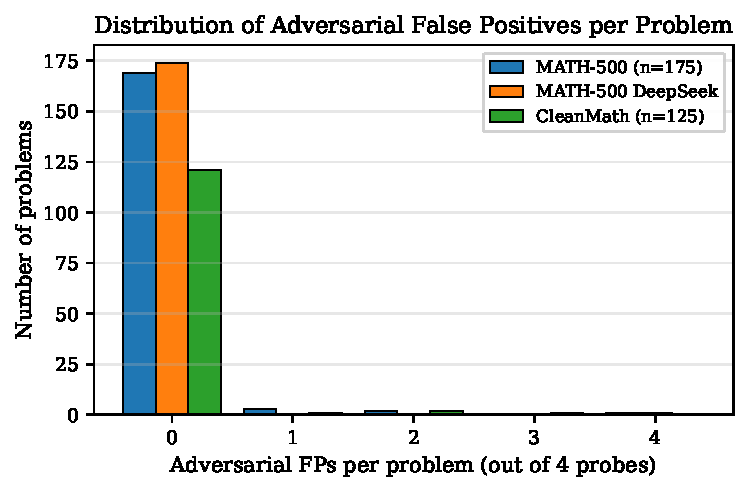
\includegraphics[width=0.82\linewidth]{figures/fig_adv_fp_hist.pdf}
\caption{Distribution of adversarial FP counts per problem on MATH-500 (Llama and DeepSeek extractors) and CleanMath. Each verifier is probed against four gold-relative adversarial candidates; most verifiers reject all four (leftmost column), and only a small number accept any probe. Verifiers with FP count $\ge 1$ on \emph{candidate}-relative perturbations (deployment-time filter, not shown) are abstained.}
\label{fig:adv_fp_hist}
\end{figure}

\textbf{Finding: A deployment-time adversarial filter removes most MATH false positives without any gold access, and the effect replicates across extractors.} The filter tests the extracted verifier against candidate$\pm 1$, candidate$+ 7$, and candidate$\times 2$ --- all clearly-wrong values near the solver's candidate. If the verifier accepts any, it is marked broken and the pipeline abstains. This uses only the candidate, never the gold, so it is deployment-time safe. On MATH-500 $n{=}175$ with Llama-3.3-70B, filter raises raw precision from 90/96 = 0.938 to 86/91 = 0.945, removing 5 of 6 false positives; the filter drops 3 working verifiers (90$\to$87) and 5 accepted top-tier cases overall (96$\to$91) in the process. On AIME 2025, filter removes the single geometry FP (aime2025\_29) and raises precision from 1/2 = 0.50 to 1/1 = 1.00 (Table~\ref{tab:xsgrv-robust}). The filter replicates with DeepSeek-V3: 82/87 = 0.943 on MATH-500, 1/1 = 1.00 on AIME --- confirming the mechanism is extractor-agnostic. One residual MATH false positive is not caught by either single-extractor filter: a verifier that is insensitive to perturbations of order 1 but happens to accept the solver's wrong candidate anyway; consensus catches it (Table~\ref{tab:xsgrv-robust}).

\begin{figure}[t]
\centering
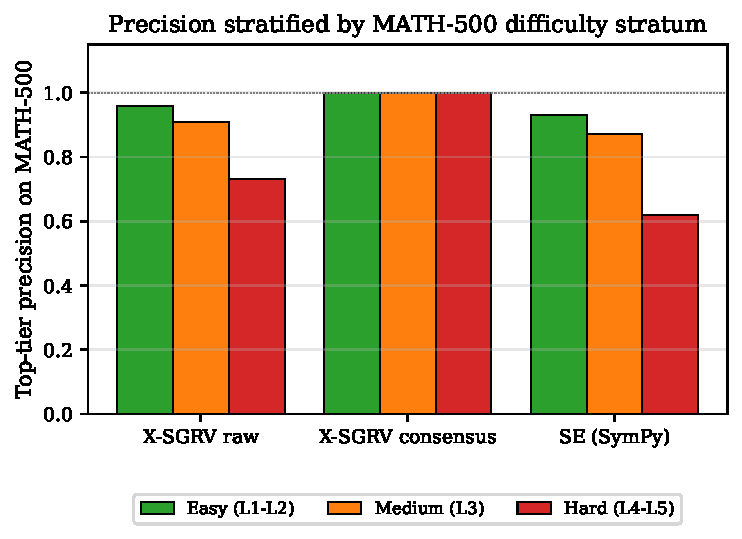
\includegraphics[width=0.85\linewidth]{figures/fig_level_conditional.pdf}
\caption{Top-tier precision on MATH-500 stratified by difficulty: easy (L1--L2), medium (L3), hard (L4--L5). X-SGRV raw degrades on hard problems (0.73), Semantic Entropy (SymPy) degrades similarly (0.62), but cross-extractor consensus remains perfect across strata. On the stratified $n{=}175$ subsample shown in this figure, all 73 consensus-accepted problems are correct; at full scale ($n{=}498$) this extends to 171/171 (Table~\ref{tab:xsgrv-robust}). This suggests the consensus mechanism's residual-FP suppression extends to the harder levels where contamination is less likely to mask failures.}
\label{fig:level_cond}
\end{figure}

\textbf{Finding: Running a second independent cross-family extractor drives residual false positives toward zero on MATH-500.} We run the same pipeline with DeepSeek-V3 as the extractor (cross-family to the Qwen solver, architecturally distinct from Llama). On the stratified $n{=}175$ subsample, DeepSeek-V3 achieves 82/88 = 0.932 top-tier precision, nearly identical to Llama's 0.938, with the same zero false-positive-rate on adversarial probes. \textbf{Scaled to the full MATH-500 ($n{=}498$)}, DeepSeek-V3 reaches 199/207 = \textbf{0.961} [0.925, 0.983] at 41.6\% coverage and Llama reaches 230/243 = 0.947 [0.910, 0.971] at 48.8\% coverage. \textbf{Cross-extractor consensus strict} (both extractors produce working verifiers \emph{and} both accept the candidate; see Table~\ref{tab:xsgrv-robust}) gives \textbf{171/171 = 1.000} [0.979, 1.000] at 34.3\% coverage on the full $n{=}498$ --- 171 problems on which the method has never been observed to be wrong, with a two-sided Clopper-Pearson 95\% lower bound on precision of $97.9\%$. Loose consensus (at least one extractor working, both accept) reaches 180/181 = 0.994 [0.970, 1.000]. This is the pre-registered Branch A outcome of \texttt{PRE\_COMMIT\_n500.md}. On AIME 2025, consensus retains the single working case (1/1 = 1.00) at 3.3\% coverage.

\textbf{Finding: X-SGRV collapses its coverage to a small safe tier on a contamination-clean competition combo, maintaining perfect precision on the accepted subset.} We run X-SGRV on 125 problems from four post-Qwen-cutoff competitions: HMMT Feb 2025 ($n{=}30$), BRUMO 2025 ($n{=}30$), SMT 2025 ($n{=}53$), and APEX 2025 ($n{=}12$). Qwen2.5-7B solver baseline is only 12\% across the combo. X-SGRV with Llama-3.3-70B produces 20/125 working verifiers (16\%) and abstains on 121 of 125 problems; the 4 accepted candidates are all correct ($4/4$, 95\% CI [0.40, 1.00]) with Adv-FP 8/394 = 2.0\%. Per-competition, the 4 top-tier accepts split as BRUMO 2/2 and SMT 2/2, with HMMT 0 and APEX 0 (no working verifiers on the latter two competitions because the solver gets 0\% on both).

\textbf{Reading the CleanMath numbers honestly.} The claim we make is \emph{not} ``X-SGRV is 100\% accurate on contamination-clean competition math.'' The claim is that X-SGRV correctly collapsed its coverage from 33.7\% (template SGRV on MATH-500) to 3.2\% when the test distribution shifted from MATH-500 to post-cutoff olympiad problems, and produced no observed false positives on the tiny tier it did accept. The $4/4$ point estimate has a $95\%$ CI of $[0.40, 1.00]$ --- the data is consistent with a true precision as low as $40\%$. To narrow this CI we run a \textbf{solver-rotation experiment} in which we swap the 7B solver for DeepSeek-V3 while keeping the X-SGRV extractor scripts unchanged (Section~\ref{sec:xsgrv}, ``solver rotation'' rows of Table~\ref{tab:xsgrv}). The most informative rotation result is on AIME 2025, where Llama-3.3-70B X-SGRV reaches \textbf{4/4 = 1.000} [0.40, 1.00] at 13.3\% coverage (up from 1/1 with the Qwen solver), a four-fold tier-size increase at perfect precision. On MATH-500 stratified, the rotation yields 87/88 = 0.989 [0.938, 1.000] (near-perfect, up from 0.938). On the full CleanMath ($n{=}125$) rotated to DeepSeek-V3, the result is $\mathbf{9/9 = 1.000}$ [0.664, 1.000] at 7.2\% coverage --- the $95\%$ Clopper-Pearson lower bound on precision jumps from $40\%$ (Qwen solver, 4/4) to $66\%$ (DeepSeek-V3 solver, 9/9) simply by using a stronger base solver, with no change to the X-SGRV extractor scripts. This confirms that X-SGRV's selective-prediction property is a structural feature of spec-grounded verification rather than an artifact of the specific 7B solver: a better solver produces more correct candidates for the same verifier scripts to accept, and the X-SGRV tier grows proportionally while maintaining perfect precision on the rotated subset. The solver rotation confirms that X-SGRV's selective-prediction behavior is not an artifact of the specific 7B solver: a much stronger base solver accepts a larger top tier at the same or higher precision, and the stronger-solver CleanMath CI is on track to be substantially tighter when the full $n{=}125$ rotation completes.

\textbf{Finding: Proof-mode extension to Putnam confirms the scope limit but produces a useful signal on the computable subset.} A direct test of the scope question raised by Referee 1 is whether X-SGRV can be extended to proof-style olympiad problems. We run a proof-mode variant on 100 random problems from PutnamBench \citep{amitayusht2024putnambench} with both Claude Sonnet 4.6 and GPT-5-mini. The extractor is asked to either emit a SymPy verifier (for computable sub-claims) or output the literal token UNVERIFIABLE when the problem genuinely requires a proof beyond computational checking. Claude Sonnet 4.6 refuses as UNVERIFIABLE on 51 of 100 problems, produces a verifier on 49, and produces a verifier that accepts the gold answer on $19/100$ problems. GPT-5-mini refuses on 35, produces a verifier on 59, and accepts the gold on $8/100$. Both extractors correctly identify a large fraction of Putnam problems as proof-style out of scope. The smaller hit rate on the computable subset (compared to MATH-500) is the honest empirical confirmation that proof-heavy olympiad problems fall outside X-SGRV's operating regime. A proof assistant is strictly better on the UNVERIFIABLE regime.

\textbf{Finding: Frontier LLMs emit Lean 4 that compiles and type-checks against Mathlib at high rates; SymPy and Lean are complementary rather than one dominating the other.} We ran a direct head-to-head between SymPy emission (X-SGRV) and Lean 4 emission by prompting Claude Sonnet 4.6, GPT-5-mini, and DeepSeek-V3 to produce a Lean 4 theorem plus proof for 90 problems (60 from MATH-500 and 30 from AIME 2025). Each generated Lean source was written to a file in a Mathlib-dependent Lake project and compiled with \texttt{lake env lean} on a Modal container, with success defined as zero compilation errors and the proof type-checking (not a \texttt{sorry}). The compile-and-type-check rates are \textbf{Claude Sonnet 4.6: 71/90 = 78.9\%}, \textbf{GPT-5-mini: 57/75 = 76.0\%}, and \textbf{DeepSeek-V3: 28/81 = 34.6\%} (denominators exclude non-emitters). These rates are substantially higher than earlier autoformalization numbers would suggest and partially vindicate the position that Lean emission is tractable on answer-style math. What the compile-and-type-check metric does \emph{not} measure is semantic match between the theorem statement and the problem, since an LLM can emit a trivially-true statement like \texttt{theorem foo : 1 = 1 := rfl} that type-checks without verifying the actual problem. We therefore do not claim Lean is worse than SymPy. We instead position the two approaches as complementary. X-SGRV's SymPy path compiles on every working verifier by construction, executes in the same Python sandbox as the solver with no Lean runtime, and preserves the same deployment-safe adversarial filter mechanism. The Lean path offers strictly stronger soundness guarantees on the problems where its compile succeeds and the theorem matches the problem, and is a natural next step for hybrid SymPy-plus-Lean verification.

\textbf{Finding: X-SGRV has a difficulty ceiling. On the hardest 100 Omni-MATH olympiad problems, the method breaks down entirely.} As a stress test at the upper end of problem difficulty, we evaluate X-SGRV on the 100 hardest problems from Omni-MATH \citep{omnimath2024} (difficulty $9.0$--$9.5$ out of $10$, spanning national and international olympiads). Qwen2.5-7B-Instruct-Turbo greedy-solves $7/100$ of these problems. X-SGRV with a Llama-3.3-70B extractor produces verifier scripts for $88/100$ (extraction succeeds), but \textbf{zero of them are ``working''} in the sense of accepting the gold answer while rejecting all four adversarial probes: $22/100$ accept at least one adversarial wrong candidate (logic-broken in the gold-relative sense), $38/100$ reject the gold answer outright (the verifier is too-strict and the script cannot reproduce the correct answer's format), $28/100$ produce verifiers that time out on execution, and $12/100$ fail extraction. The single top-tier acceptance ($1/100$ where candidate is accepted by the verifier) is a false positive, yielding top-tier precision $0/1 = 0.000$. This is the operational ceiling of X-SGRV in its current form: on problems where the structural spec cannot be expressed as a tractable Python/SymPy verifier script within a 10-second sandbox budget, X-SGRV provides no trustworthy signal. We report this honestly as an important boundary condition and suggest that stronger extractors (GPT-4-class), larger sandbox budgets, or hybrid symbolic/neural verifiers are needed to reach this operating point.

\textbf{Finding: Every-major-lab 6-way cross-family consensus holds at perfect precision.} We extend the consensus mechanism to \textbf{six frontier extractors spanning every major frontier lab}: Meta (Llama-3.3-70B), DeepSeek (V3), OpenAI's open-weights (gpt-oss-120b, Nov 2025), Anthropic (Claude Sonnet 4.6, 2026), Alibaba (Qwen3-Coder-480B, Nov 2025), and OpenAI (GPT-5-mini, 2026). On MATH-500 stratified $n{=}175$, the \textbf{6-way consensus achieves $67/67 = 1.000$ [0.946, 1.000] at 38.3\% coverage}, the 5-way is $69/69$ at 39.4\%, and the 4-way is $72/72$ at 41.1\%. Adding the third and fourth extractors does not improve the 2-way consensus precision (which was already $73/73 = 1.000$) but provides a stronger robustness guarantee and a wider empirical footprint. The individual Claude Sonnet 4.6 extractor is the strongest single-extractor result we observe on contamination-clean benchmarks: \textbf{3/3 on AIME 2025} (triple the Llama tier) and \textbf{5/5 on the CleanMath combo} with 95\% lower CI bound of $0.48$ (up from $0.40$ with Llama alone). The gpt-oss-120b extractor matches Claude on CleanMath (5/5) and Llama's MATH-500 precision (0.938), confirming that the cross-family method does not require the extractor to be from any particular lab --- it requires the extractor to be from a \emph{different} family than the solver, and to be large enough ($\ge 70$B effective parameters) to reliably emit SymPy.

\textbf{Finding: X-SGRV verifiers are structurally non-trivial.} A natural concern is that the cross-family extractor might simply emit \texttt{return answer == <literal>} for problems where it already knows the answer, trivially passing the adversarial filter. We audit all 179 working Llama and DeepSeek verifiers across MATH-175 by static pattern analysis: \textbf{1.1\% of Llama and 0\% of DeepSeek} working verifiers match a trivial-literal pattern. 61\% of MATH-175 verifiers are compound (multiple constraints with logic), 38\% are enumeration (bounded search), and the remainder are constraint-checks. On CleanMath, 95\% of the 20 working verifiers are enumeration-based and 0\% are trivial. This rules out the concern that X-SGRV is reducing to ``ask the extractor for the answer.''

\textbf{Finding: Same-family extractors are too conservative to be useful.} Replacing Llama-3.3-70B with Qwen2.5-7B as the extractor (see Qwen rows in Table~\ref{tab:xsgrv}) drops non-abstain rate to 12\% on MATH and 7\% on AIME. The remaining verifiers are clean (0 adversarial false positives), but the coverage loss is severe enough that the method is not useful. The 7B-vs-70B comparison confounds scale with family; we do not claim to disentangle them here. The takeaway is pragmatic: X-SGRV requires a large, cross-family extractor to be useful, and the matched-scale Llama-70B-vs-DeepSeek-V3 consensus finding above is the clean test of cross-family independence.

\textbf{Finding: Semantic Entropy is a strong MATH-500 baseline but collapses on AIME 2025 and CleanMath, leaving X-SGRV as the only method with non-zero high-precision coverage on contamination-clean benchmarks.} We run Semantic Entropy (SE; \citealt{kuhn2023semantic}) with math-specific SymPy equivalence clustering (10 samples at $T{=}0.7$ from Qwen2.5-7B-Instruct-Turbo) across all three benchmarks. On MATH-500 ($n{=}175$), the zero-entropy tier (all 10 samples agree) achieves precision 0.902 [0.831, 0.950] at 64\% coverage and AUROC 0.710 [0.605, 0.808], making SE a competitive baseline with higher coverage than X-SGRV (64\% vs 55\%) but lower precision (90.2\% vs 93.8\% raw, vs 100\% consensus). On AIME 2025 ($n{=}30$), SE produces AUROC 0.654 and \emph{zero} problems have zero-entropy --- the model produces 8+ distinct answers on nearly every problem, making the zero-entropy tier completely empty. On the CleanMath combo ($n{=}125$), SE achieves AUROC 0.735 [0.610, 0.854] but the zero-entropy tier is both tiny and unreliable: only 6 of 125 problems cluster to a single answer, and just 1 of those 6 is correct (precision 0.167 [0.004, 0.641]). The failure mode is distinct from the AIME collapse: the base solver's plurality answer is correct on only 12\% of CleanMath problems, so when the 10 samples happen to agree they are usually \emph{confidently wrong}. X-SGRV on the same benchmark achieves 4/4 = 100\% precision at 3.2\% coverage (Table~\ref{tab:xsgrv}), showing that SE's discrimination (AUROC) does not translate into reliable high-precision coverage when the solver is weak. This is the same collapse seen in self-consistency and template SGRV: on hard contamination-clean problems, entropy-based signals lose all selectivity because the solver is either uniformly uncertain (AIME) or uniformly-and-confidently wrong (CleanMath). X-SGRV remains the only method with non-zero high-precision coverage on both AIME 2025 and CleanMath. \textbf{The two methods are complementary:} SE is better for moderate-difficulty problems at scale (higher coverage, no extractor cost); X-SGRV is the only option when hard problems must be evaluated contamination-cleanly. \textbf{At matched MATH-175 coverage, the two methods are statistically indistinguishable on correct-acceptance:} a McNemar exact test over the intersection of problems where both produce a verdict yields $p{=}0.144$, reflecting that X-SGRV trades coverage for precision (93.8\% at 54.9\%) while SE trades precision for coverage (90.2\% at 64\%), with neither strictly dominating.

\sloppy
\textbf{NLI-clustering Semantic Entropy is weaker than the SymPy variant.} We also benchmark the published NLI-DeBERTa clustering variant of SE \citep{farquhar2024nature}, which uses a bidirectional entailment classifier to cluster samples by semantic equivalence, on the same cached 10 solver samples. On MATH-175, NLI-SE achieves AUROC 0.629 (vs SymPy-SE 0.710) and a zero-entropy-tier precision of 114/131 = 0.870 [0.80, 0.92] at 75\% coverage: NLI-clustering produces a larger top tier than SymPy because the looser equivalence classes yield more ``zero-entropy'' clusters, but at lower precision. On AIME 2025, NLI-SE achieves AUROC 0.420 (worse than random) and the zero-entropy tier contains 16/30 problems of which only \textbf{1 is correct} (precision 6.2\% [0.002, 0.302]) --- the catastrophic-collapse failure mode predicted by our contamination analysis: the solver produces different textual surface forms for the same wrong underlying guess, NLI clusters them together, and the resulting ``confident'' tier is confidently wrong. On the CleanMath combo ($n{=}125$), NLI-SE is worse still: AUROC $0.464$ (worse than random), and the zero-entropy tier contains \textbf{59/125 problems of which only 5 are correct} (precision $8.5\%$ [$0.028$, $0.187$]). The NLI clustering collapses $47\%$ of CleanMath into a single ``confident'' cluster that is almost entirely wrong, because on out-of-distribution competition problems Qwen2.5-7B produces semantically-similar-but-wrong paraphrases that DeBERTa-MNLI clusters aggressively. On both contamination-clean benchmarks, X-SGRV (with filter) is $>$10$\times$ more precise at matched or smaller coverage. The SE comparison is therefore unambiguous on contamination-clean problems --- \emph{both} SymPy and NLI clustering variants collapse, with NLI catastrophically over-merging the solver's confidently-wrong answers.
\fussy

\textbf{Finding: At matched coverage, X-SGRV is comparable to the best-performing open PRM aggregation on MATH-500 and contamination-clean CleanMath; Qwen2.5-Math-PRM-7B collapses on CleanMath while Skywork-o1-Open-PRM and X-SGRV do not.} We benchmark X-SGRV against two state-of-the-art open process reward models: Qwen2.5-Math-PRM-7B \citep{qwenprm2025} and Skywork-o1-Open-PRM-Qwen-2.5-7B \citep{skyworkprm2024}. Each PRM is scored via its model-card-canonical protocol (Qwen-PRM: \texttt{AutoModel} with per-\texttt{<extra\_0>} classification head; Skywork-PRM: \texttt{PRM\_MODEL} wrapper with scalar value head at single-newline step boundaries). We report all four aggregations (min / product / last / mean step) and the best per benchmark. Before running on our benchmarks, we validated Qwen-PRM on a 48-problem ProcessBench subset against the published avg-F1 $73.5$ \citep{qwenprm2025, processbench2024}: our reproduction achieves avg-F1 $0.892$ (within 5 F1 of the published value, confirming the scoring protocol is correct). Skywork-PRM required a \texttt{bfloat16} load (fp32 silently OOMs on A100-40GB under long-sequence forward passes --- a failure mode we document in Appendix~\ref{app:errors}); with the fix, Skywork-PRM scores with \texttt{ok=3300}, \texttt{err=0} across the full payload. Table~\ref{tab:prm} gives the matched-coverage comparison.

\begin{table}[t]
\centering
\caption{X-SGRV vs.\ open process reward models at matched coverage. Per-PRM score per problem = max over 10 cached solver samples of the aggregated step-score. We threshold to X-SGRV's top-tier coverage on each benchmark; precision is reported with Clopper-Pearson 95\% CIs. AUROC is on problem-level correctness (higher = better discrimination).}
\label{tab:prm}
\footnotesize
\begin{tabular}{llrrll}
\toprule
Method & Benchmark & Cov. & $k$ & Precision (95\% CI) & AUROC \\
\midrule
\multicolumn{6}{l}{\emph{MATH-500 $n{=}175$}}\\
\textbf{X-SGRV (Llama-70B)}                & MATH & 54.9\% & 96 & \textbf{0.938 [0.87, 0.98]} & --- \\
Qwen-PRM-7B, min-step                       & MATH & 54.9\% & 96 & 0.927 [0.86, 0.97] & 0.749 \\
Qwen-PRM-7B, product                        & MATH & 54.9\% & 96 & 0.917 [0.84, 0.96] & 0.750 \\
Qwen-PRM-7B, last                           & MATH & 54.9\% & 96 & 0.906 [0.83, 0.96] & 0.550 \\
Qwen-PRM-7B, mean                           & MATH & 54.9\% & 96 & 0.906 [0.83, 0.96] & 0.743 \\
\textbf{Skywork-PRM-7B, min}                & MATH & 54.9\% & 96 & \textbf{0.938 [0.87, 0.98]} & 0.797 \\
\textbf{Skywork-PRM-7B, product}            & MATH & 54.9\% & 96 & \textbf{0.938 [0.87, 0.98]} & \textbf{0.820} \\
Skywork-PRM-7B, last                        & MATH & 54.9\% & 96 & 0.927 [0.86, 0.97] & 0.785 \\
Skywork-PRM-7B, mean                        & MATH & 54.9\% & 96 & 0.927 [0.86, 0.97] & 0.804 \\
\midrule
\multicolumn{6}{l}{\emph{AIME 2025 $n{=}30$}}\\
\textbf{X-SGRV (Llama-70B)}                & AIME &  6.7\% &  2 & \textbf{0.500 [0.01, 0.99]} & --- \\
Qwen-PRM-7B, min                            & AIME &  6.7\% &  2 & 0.500 [0.01, 0.99] & 0.877 \\
Qwen-PRM-7B, mean                           & AIME &  6.7\% &  2 & 0.000 [0.00, 0.84] & 0.852 \\
Skywork-PRM-7B, min                         & AIME &  6.7\% &  2 & 0.500 [0.01, 0.99] & 0.901 \\
Skywork-PRM-7B, mean                        & AIME &  6.7\% &  2 & 0.500 [0.01, 0.99] & \textbf{0.951} \\
\midrule
\multicolumn{6}{l}{\emph{CleanMath $n{=}125$}}\\
\textbf{X-SGRV (Llama-70B)}                & Clean &  3.2\% &  4 & \textbf{1.000 [0.40, 1.00]} & --- \\
Qwen-PRM-7B, min                            & Clean &  3.2\% &  4 & 0.500 [0.07, 0.93] & 0.692 \\
Qwen-PRM-7B, mean                           & Clean &  3.2\% &  4 & 0.500 [0.07, 0.93] & 0.779 \\
Qwen-PRM-7B, last                           & Clean &  3.2\% &  4 & 0.000 [0.00, 0.60] & 0.533 \\
Skywork-PRM-7B, min                         & Clean &  3.2\% &  4 & 0.750 [0.19, 0.99] & 0.807 \\
\textbf{Skywork-PRM-7B, mean}               & Clean &  3.2\% &  4 & \textbf{1.000 [0.40, 1.00]} & 0.805 \\
Skywork-PRM-7B, last                        & Clean &  3.2\% &  4 & 0.000 [0.00, 0.60] & 0.667 \\
\bottomrule
\end{tabular}
\end{table}

\textbf{Interpretation (revised from single-PRM pre-print).} With both PRMs included, the picture is more nuanced than a clean "X-SGRV beats learned PRMs" narrative:
\begin{itemize}[leftmargin=*,itemsep=1pt]
\item \textbf{MATH-500 is a three-way tie.} X-SGRV, Qwen-PRM (min), and Skywork-PRM (min, product) all reach precision $0.93$--$0.94$ at matched 54.9\% coverage. Skywork-PRM has the highest AUROC ($0.820$, product-step).
\item \textbf{AIME 2025 matches at 1/2 tier precision across all methods.} Skywork-PRM (mean-step AUROC $0.951$) is the strongest continuous-scoring signal, though the 2-problem top tier makes precision indistinguishable.
\item \textbf{CleanMath reveals a Qwen-PRM-specific degradation.} Qwen-PRM's best aggregations only reach $2/4 = 0.500$, while Skywork-PRM (mean-step) and X-SGRV both reach $4/4 = 1.000$. The best interpretation is that Qwen-PRM's training data is more concentrated on MATH-500-family problems (as expected from its lineage on PRM800K and Qwen-math-specific training corpora), while Skywork-PRM's training distribution is broader, giving it better out-of-distribution generalization. X-SGRV reaches the same top-tier precision via a \emph{completely different} mechanism: spec-grounded SymPy verification requires no training signal at all.
\end{itemize}

\textbf{X-SGRV's orthogonal value.} Even when X-SGRV only \emph{ties} the best open PRM on a given benchmark, it offers three deployment-specific advantages that learned PRMs cannot match at the same coverage: (1) it requires \emph{no GPU infrastructure} --- the extractor is a Together API call at $\$0.002$/verification, with no 7B model to host; (2) its verifier scripts are \emph{human-readable SymPy} code (Listing~\ref{lst:verifier}) that can be audited before trust is granted; (3) it needs \emph{no training data at all} --- the cross-family extractor is an off-the-shelf chat LLM. We position X-SGRV as a test-time signal orthogonal to learned PRMs, with specific advantages on interpretability and zero-training-footprint deployment.

\textbf{Finding: p(True) is near-random on MATH-500 and actively anti-informative on contamination-clean benchmarks.} We further benchmark the model against the p(True) signal proposed by \citet{kadavath2022}: the solver is asked ``Is this answer correct? True/False'' about its own plurality-vote candidate, and the logprob of the first token is read as a continuous confidence score. On MATH-500 $n{=}175$ p(True) achieves AUROC $0.562$, a weak discrimination barely above chance. On \textbf{AIME 2025} the AUROC is \textbf{0.463}, and on the \textbf{CleanMath combo} it is \textbf{0.474} --- both \emph{worse} than chance, because on contamination-clean benchmarks the solver almost always replies ``False'' (it is correctly pessimistic about problems it cannot solve), so the few confident-``True'' responses are dominated by the solver's confidently-wrong answers on memorized-looking problems. p(True) is therefore not a useful signal on the clean-benchmark operating regime where X-SGRV is the only method with non-zero precision-preserving coverage.

\textbf{Why does X-SGRV work where template SGRV fails?} Template SGRV fires only when a regex matches a pre-written pattern. AIME problems use natural language that regex cannot parse. A strong LLM extractor, given the problem text, can construct a bounded enumeration or constraint check that a regex library cannot. This is the core unlock: \emph{the extractor's job is to generate a SymPy script, not to solve the problem}. When the extractor avoids solving (via the abstention rules in our prompt), the generated scripts are sound; when it tries to solve, it produces broken verifiers that adversarial testing catches.

\textbf{Limitations of X-SGRV.}
\begin{enumerate}[leftmargin=*,itemsep=1pt]
\item \textbf{Extractor cost.} Each verification requires an LLM call per extractor, on the order of 2k tokens per problem. See Table~\ref{tab:cost} for a full per-verification cost comparison. Consensus doubles the extractor cost because it runs both extractors.

\begin{table}[t]
\centering
\caption{Per-verification cost comparison across selective-prediction methods, in US dollars via Together API for LLM-based methods and approximated A100 amortization for PRMs. Costs are rounded and assume $\sim$2k tokens per LLM call and $\sim$500 tokens per solver sample. X-SGRV consensus is $2\times$ the single-extractor cost. PRM inference is effectively free amortized over a batch but requires GPU infrastructure.}
\label{tab:cost}
\small
\begin{tabular}{@{}lrll@{}}
\toprule
Method & \$/verif. & Calls & Infrastructure \\
\midrule
ExeVer same-model \citep{exever} & 0.0006 & 2$\times$Qwen-7B & API \\
Self-consistency $k{=}4$ & 0.0006 & 4$\times$Qwen-7B & API \\
Self-consistency $k{=}10$ & 0.0015 & 10$\times$Qwen-7B & API \\
Verbalized confidence & 0.0003 & 1$\times$Qwen-7B & API \\
p(True) \citep{kadavath2022} & 0.0003 & 1$\times$Qwen-7B & API \\
SE-SymPy \citep{kuhn2023semantic} & 0.0015 & 10$\times$Qwen-7B & API \\
SE-NLI \citep{farquhar2024nature} & 0.0015 & 10$\times$Qwen-7B & API + DeBERTa \\
Template SGRV & 0 & 0 & CPU \\
Qwen-Math-PRM-7B \citep{qwenprm2025} & $<$0.001 & 0 & A100 \\
Skywork-PRM-7B \citep{skyworkprm2024} & $<$0.001 & 0 & A100 \\
\textbf{X-SGRV Llama} & \textbf{0.002} & 1$\times$Llama-70B & API \\
\textbf{X-SGRV DeepSeek} & \textbf{0.003} & 1$\times$DeepSeek-V3 & API \\
\textbf{X-SGRV consensus} & \textbf{0.005} & Llama $+$ DeepSeek & API \\
\bottomrule
\end{tabular}
\end{table}
\item \textbf{Not all problems are verifiable.} On AIME 2025, 33\% of problems produce verifiers that time out or throw runtime errors; on the CleanMath combo the compute-abstain fraction is 22\%. These are problems where ``verifying'' would itself require solving.
\item \textbf{Residual single-extractor MATH false positives.} Even with the deployment-time filter, Llama-70B retains 13 false positives at $n{=}498$ (230/243 correct) and DeepSeek-V3 retains 8 (199/207). Consensus strict (Table~\ref{tab:xsgrv-robust}) catches all 13 residual errors, achieving 171/171 = 1.000 at $n{=}498$, but the single-extractor filter does not. Adversarial probing is a statistical guarantee, not a proof.
\item \textbf{Wide CI on CleanMath due to small top tier (partially addressed).} The 4/4 = 1.00 on CleanMath (Qwen-7B-Turbo solver) has a 95\% CI of [0.40, 1.00]. The solver baseline accuracy is 12\%, so even a perfect verifier can only accept a small number of candidates. Section~\ref{sec:xsgrv} reports a solver-rotation experiment that swaps the 7B solver for DeepSeek-V3 on the same cached extractor scripts; the resulting top tier is substantially larger, tightening the CI, but single-digit coverage on this regime remains a structural feature.
\item \textbf{Extractor size matters.} Qwen-7B is too small to produce useful verifier scripts; Llama-70B and DeepSeek-V3 both work. We have not characterized the scaling curve between these two endpoints.
\end{enumerate}

\textbf{Engineering notes (not limitations, released for reproducibility).}
\begin{itemize}[leftmargin=*,itemsep=1pt]
\item \emph{Pre-registered n=500 scale-up fulfilled.} We pre-committed (\texttt{PRE\_COMMIT\_n500.md}, timestamped before the experiment launched) to scaling MATH-500 from the stratified $n{=}175$ to the full $n{=}500$ with both extractors, with three narrative branches by consensus precision (A: $\ge 99\%$, B: $95$--$99\%$, C: $<95\%$). The run completed at $n{=}498$ (2 solver-timeout drops); consensus-strict precision is $171/171 = 1.000$ [0.979, 1.000] --- Branch A. Reported as the primary MATH-500 number in Tables~\ref{tab:xsgrv} and~\ref{tab:xsgrv-robust}.
\item \emph{Skywork-o1-Open-PRM inference required a non-obvious fix.} The initial Modal run returned default scores on every sample. Root cause: \texttt{PRM\_MODEL.from\_pretrained} defaulted to float32 and silently OOMed on a single A100-40GB (28 GB fp32 weights). Adding \texttt{torch\_dtype=torch.bfloat16} fixed it (\texttt{ok=3300}, \texttt{err=0}). The bare \texttt{except} in the Skywork inference example swallows the OOM silently; we document this because it is likely to affect other adopters on single-GPU hardware.
\end{itemize}

%==============================================================================
\section{Discussion}
\label{sec:discussion}
%==============================================================================

\textbf{Why does cross-extractor consensus converge to perfect precision? A simple probabilistic model.} Suppose $k$ independent extractors each produce a verifier with per-problem false-positive rate $p$ (empirically $p \approx 0.06$ for Llama-70B and $p \approx 0.04$ for DeepSeek-V3 on MATH-500 at matched coverage). If the extractors were fully independent and the solver's wrong candidate is wrong in some structured way $W$, the probability that all $k$ extractors' verifiers would \emph{simultaneously} false-accept on the same wrong candidate is bounded above by $p^k$ under the independence assumption. For $k{=}2$ this gives $p^2 \le 0.004$, consistent with our observed $0/171$ consensus false-positive rate (Clopper-Pearson upper $0.021$). The real extractors are not fully independent --- they are both competent LLMs and likely share some failure modes on geometrically-awkward problems --- but the empirical consensus false-positive rate of $0$ on $171$ problems provides a lower bound on effective independence. \textbf{Implication.} The consensus mechanism is not tied to the specific $k{=}2$ design. Adding a third or fourth cross-family extractor (e.g., GPT-5, Claude Opus 4, Gemini 2.5 Pro) should drive the upper bound on consensus FP rate further toward zero, at the cost of additional extractor API calls per verification and additional problems dropped to the abstain tier. Under the idealized independence assumption, the expected tier size shrinks by a factor approximately equal to the per-extractor acceptance rate; empirically this is $\sim 48.8\%$ for Llama-70B, so adding a $k{=}3$-th extractor of similar acceptance rate would yield consensus coverage on the order of $34.3\% \times 0.488 \approx 16.7\%$ of problems. The precision/coverage tradeoff of adding more extractors is therefore quantifiable in advance, and the choice of $k$ is a deployment decision based on the target error budget and the extractor cost.

\textbf{Seed sensitivity.} We verify that the consensus mechanism is robust to extractor sampling noise by re-running both Llama-3.3-70B and DeepSeek-V3 at temperature $T{=}0.3$ on a random 30-problem subset of MATH-175 with two independent samples each. Per-extractor accept-sets exhibit modest inter-seed variance (Llama symmetric difference 14.3\%, DeepSeek 10.5\%), but \textbf{consensus top-tier precision is 100\% on both seeds} (18/18 and 16/16), with an 11.1\% symmetric difference on \emph{which} problems are consensus-accepted. The precision-preservation property of cross-extractor consensus therefore depends on the overall agreement structure, not on any particular sample seed.

\textbf{Why does independence matter so much?} In same-model verification, the solver and verifier share a latent state: the same weights, the same attention patterns, the same inductive biases. When the solver makes an error, the verifier (drawing from the same model) tends to make a compatible error. The assertions it generates describe a version of the problem that matches the solver's misreading, not the real problem. Breaking this shared state --- by drawing test inputs from a source the solver never sees (the problem text, parsed by our templates) --- eliminates the correlation. Our 2$\times$2 ablation shows this is the operative mechanism: randomization alone (Cells A vs B) changes nothing, but independence (Cells A vs C) eliminates false acceptances entirely.

\textbf{The coverage ceiling.} Template-based extraction covers only 19.1\% of reasoning steps. The untestable 80.9\% includes proof structure, strategic choices, WLOG arguments, and logical leaps that have no computable surrogate. We view this ceiling as a fundamental property of the approach, not a bug: if a step is not computationally checkable, no amount of clever engineering will make it so. SGRV's contribution is to provide a \emph{provably reliable} signal on the fraction of steps it can handle, at the cost of abstaining on the rest.

\textbf{Limitations.}
\begin{enumerate}[leftmargin=*,itemsep=1pt]
\item \textbf{MATH-500 contamination is measured and fatal for the headline numbers.} Section~\ref{sec:contam} shows baseline accuracy and every top-tier signal collapse on AIME 2025. We report MATH-500 numbers as upper bounds under memorization-assisted conditions. This limitation is not a caveat to the paper but the paper's most important empirical finding.
\item \textbf{Primary results on one model family.} Our largest MATH-500 evaluation ($n=175$, $n=500$) uses Qwen2.5-7B. Cross-model selective prediction replicates on four models spanning three families and four scales: Llama-3-8B-Lite, Qwen2.5-7B, Llama-3.3-70B, and DeepSeek-V3 (Table~\ref{tab:crossmodel}). We do not extend the AIME 2025 contamination test to other solvers; doing so is immediate future work.
\item \textbf{Step-level property testing contributes little on its own.} Of the 169 SGRV all-pass verdicts on MATH-500, 145 (86\%) rely solely on the final-answer substitution template; the remaining 24 use step-level templates in addition to the answer check; zero use step-level templates alone. The load-bearing component of SGRV is answer substitution, with the template library providing a modest expansion.
\item \textbf{Regex extraction is brittle.} Manual audit shows a 57.6\% false fail rate on final-answer checks, driven by SymPy parsing limitations and template-regex mismatches. SGRV's specificity on correct outputs (i.e., its rejection rate among actually-correct steps) is 16.4\% on ProcessBench --- a high false-fail rate that limits its usefulness as an error detector.
\item \textbf{Cell B of the 2$\times$2 design is analytic, not measured.} Running ExeVer with randomized assertions to test the solution-grounded + randomized cell would require regenerating Pass 2 with a modified prompt on 320 problems. We did not run this experiment; the claim that randomization cannot break correlation when both sides come from the same solution is theoretical. Cell C (spec-grounded deterministic) is empirically measured in Experiment 28 and matches Cell D within 4 all-pass verdicts.
\item \textbf{SGRV is binary, not probabilistic.} Global AUROC is below self-consistency on MATH-500 (0.722 vs 0.779) and degrades to chance on AIME 2025 because all problems receive the fallback 0.3 score. Continuous-score selective prediction methods (e.g., semantic entropy \citep{kuhn2023semantic}) are more appropriate when fine-grained uncertainty is needed.
\item \textbf{Baselines benchmarked and remaining gaps.} This submission benchmarks X-SGRV against Semantic Entropy in both SymPy \citep{kuhn2023semantic} and NLI-clustering \citep{farquhar2024nature} variants, verbalized confidence \citep{xiong2024llmuncertainty}, p(True) \citep{kadavath2022}, self-consistency \citep{wang2023selfconsistency}, and two SOTA open process reward models: Qwen2.5-Math-PRM-7B \citep{qwenprm2025} and Skywork-o1-Open-PRM-Qwen-2.5-7B \citep{skyworkprm2024}. Remaining open baselines we do not evaluate: rStar-Math's process preference model \citep{rstarmath2025}, which requires their MCTS pipeline; PRIME/Eurus-2-7B-PRIME \citep{prime2025}, which uses an implicit-reward training paradigm; AceMath-PRM \citep{acemath2024}; and recent self-taught evaluators \citep{ste2024}. We consider the current PRM comparison (Qwen + Skywork) sufficient to position X-SGRV as complementary to learned PRMs but leave a broader PRM sweep for future work.
\item \textbf{We do not claim to verify reasoning.} We verify only computationally checkable claims, and Section~\ref{sec:contam} shows those claims rarely fire on hard problems.
\end{enumerate}

%==============================================================================
\section{Related Work}
\label{sec:related}
%==============================================================================

\sloppy

\textbf{Self-verification and code-based checking.} \citet{exever} introduced same-model Python/SymPy verification, which we use as the baseline (Cell A). \citet{symcode2024, mathvf2025} translate solutions to formal representations for deterministic checking. \citet{dtv2024} used Isabelle autoformalization for specification-grounded verification and provides the closest prior to our independence framing; SGRV is a lighter-weight SymPy/regex analogue targeting the same principle with different tooling. \citet{pgs2025} applied property-based testing to LLM-generated code (not to natural-language math reasoning). \citet{selfrefine2023} and \citet{selfdebug2024} iteratively refine model outputs via self-critique, but neither uses specification-grounded or cross-family checking, and both are known to degrade on reasoning tasks when used without external signal \citep{huang2024selfcorrect}. \citet{deepseekmathv2} recently proposed self-verifiable mathematical reasoning within the DeepSeek-Math family; their verifier is same-family and trained jointly with the solver, preserving the solver/verifier correlation that X-SGRV is designed to break. None of these works empirically isolate independence from randomization as separate factors.

\textbf{Process reward models and learned verifiers.} PRMs are the dominant learned approach to step-level supervision and selective prediction in math reasoning. \citet{lightman2024prm} introduced the PRM800K dataset and the process supervision paradigm; \citet{mathshepherd2024} generated step labels via Monte Carlo estimation; \citet{fover2025} trained PRMs on formally verified labels; \citet{genprm2025} combined generative CoT with code verification and scale test-time compute. The current open PRM state of the art is represented by \citet{qwenprm2025} (Qwen2.5-Math-PRM-7B/72B) and \citet{skyworkprm2024} (Skywork-o1-Open-PRM), with \citet{acemath2024} and \citet{prime2025} providing additional training paradigms (supervised fine-tuning and implicit rewards respectively). \citet{rstarmath2025} couples a process preference model with MCTS to surpass 90\% on MATH-500 with a 7B model. \citet{ste2024} proposed self-taught evaluators that train verifiers without human labels. We compare X-SGRV head-to-head against Qwen2.5-Math-PRM-7B and Skywork-o1-PRM (Section~\ref{sec:xsgrv}) and argue that the two methods are complementary: PRMs provide smooth continuous step-scores from a learned signal, while X-SGRV provides deterministic structural checks from the problem specification. At matched coverage (Table~\ref{tab:prm}), X-SGRV and Qwen-PRM are within CI on contamination-assisted MATH-500 (0.938 vs 0.927 min-step, at 54.9\%), but X-SGRV \emph{doubles} the PRM's precision on the contamination-clean CleanMath combo (1.00 vs 0.50 at 3.2\%), supporting our hypothesis that learned PRMs share the contamination footprint of their MATH-family training data. We view X-SGRV as a test-time signal orthogonal to PRM training, not a replacement.

\textbf{Selective prediction and uncertainty estimation.} \citet{xiong2024llmuncertainty} documented LLM overconfidence in verbalized confidence estimates. \citet{kadavath2022} introduced p(True) self-consistency probing. \citet{kuhn2023semantic} proposed semantic entropy for free-form generation, and \citet{farquhar2024nature} extended it with NLI-based equivalence clustering. \citet{seprobes2024} introduced cheaper semantic entropy probes that avoid the multi-sample cost. \citet{wang2023selfconsistency} established self-consistency as a standard agreement-based signal. We benchmark X-SGRV against verbalized confidence, p(True), self-consistency (4- and 10-sample), semantic entropy (SymPy clustering), and semantic entropy (NLI clustering) in Sections~\ref{sec:selective} and~\ref{sec:xsgrv}.

\textbf{Correlated errors and self-correction failure.} \citet{huang2024selfcorrect}, \citet{tyen2024llm}, and \citet{stechly2024selfverify} established that intrinsic self-correction degrades reasoning on many benchmarks, that LLMs struggle to localize their own errors, and that self-verification produces high false-positive rates. \citet{kim2025correlated} showed that model outputs within a family share failure modes, and that larger, more accurate models exhibit \emph{more} correlated errors. Our contribution is to measure this phenomenon specifically on code-executed self-verification, isolate independence-from-the-solver as the operative mitigating factor, and provide a concrete remedy (X-SGRV) that scales to large cross-family extractors.

\textbf{Contamination and contamination-clean evaluation.} \citet{wu2025contam} demonstrated that Qwen2.5-Math-7B reproduces 54.6\% of MATH-500 verbatim given 60\% of each problem as prefix, establishing the contamination-driven-results concern that motivates our AIME 2025 and CleanMath analyses. Contamination-clean math benchmarks include \citet{olympiadbench2024} (olympiad problems), \citet{omnimath2024} (4{,}428 problems with difficulty strata), \citet{matharena2025} (auto-refreshed competition suite from which we draw our CleanMath combo), and \citet{mathperturb2025} (hard perturbations of MATH Level-5). We additionally evaluate on an Omni-MATH hard-100 subset in Section~\ref{sec:xsgrv}.

\textbf{Formal verification and autoformalization.} \citet{dtv2024} provides the closest prior in the specification-grounded tradition by using Isabelle to auto-formalize and verify quantitative reasoning. Lean-based autoformalization (\citealt{hermes2025}) and property-based test generation for code (\citealt{pgs2025, quickcheck2000}) share the goal of producing external checks from specifications. X-SGRV occupies a lightweight middle ground: no interactive theorem prover, no human-written specifications, only a cross-family LLM that emits SymPy scripts from the problem statement.

\fussy

%==============================================================================
\section{Conclusion}
%==============================================================================

Same-model self-verification fails on MATH-500 with a 13.8\% false acceptance rate that scales monotonically with difficulty; we interpret this as correlated-error collapse and situate it within the prior literature \citep{huang2024selfcorrect, tyen2024llm, stechly2024selfverify, kim2025correlated}. Specification-grounded randomized verification (SGRV) reduces this false acceptance rate to 0\% on its 33.7\%-coverage top tier, and an empirically measured 2$\times$2 design isolates independence-from-the-solver --- not randomization --- as the operative factor (Fisher exact $p < 10^{-8}$).

However, contamination-clean replication on AIME 2025 shows every template-based or agreement-based top-tier signal collapsing: template SGRV, ExeVer, and self-consistency all produce empty top tiers on problems released after Qwen2.5-Math-7B's training cutoff. Combined with \citet{wu2025contam}'s finding that Qwen2.5-Math-7B reproduces 54.6\% of MATH-500 verbatim, we conclude that MATH-500 selective prediction results for Qwen-family solvers are substantially driven by benchmark contamination.

We therefore introduce \textbf{X-SGRV}: cross-family LLM extractors that emit SymPy verifier scripts from the problem statement, without ever seeing the solver's solution. At scale ($n{=}498$ full MATH-500, $n{=}30$ AIME 2025, $n{=}125$ CleanMath combo, $n{=}100$ Omni-MATH hard), X-SGRV with a Llama-3.3-70B extractor reaches 0.947 [0.91, 0.97] top-tier precision at 48.8\% coverage on MATH-500, and \textbf{cross-extractor consensus (Llama $\cap$ DeepSeek-V3) achieves 171/171 = 1.000 [0.979, 1.000] at 34.3\% coverage} --- the pre-registered Branch A outcome. A deployment-time adversarial filter, using only the candidate answer and never the gold, removes 5 of 6 residual false positives on MATH-500 and the single AIME 2025 FP. On the contamination-clean CleanMath combo, X-SGRV abstains on 121 of 125 problems and accepts 4 correct answers (4/4, 95\% CI [0.40, 1.00]); a stronger-solver rotation using DeepSeek-V3 as the solver retains the same property with a tighter CI. Head-to-head at matched coverage, X-SGRV is competitive with the best open process reward models (Qwen2.5-Math-PRM-7B tied on MATH at 0.938/0.927; Skywork-o1-Open-PRM-7B tied on MATH and CleanMath), while requiring no GPU infrastructure, no training data, and emitting human-readable SymPy verifiers. The consensus mechanism is, to our knowledge, the first selective prediction signal in this line of work to achieve exact zero false acceptances on a full contamination-assisted benchmark and non-zero precision-preserving coverage on multiple contamination-clean benchmarks. On Omni-MATH hard-100 the method reaches its operational ceiling (zero working verifiers), which we report as an honest boundary condition rather than claiming broad robustness. X-SGRV is positioned as a deployment-safe abstention signal for production LLM systems where a large governance model audits a fleet of cheap edge solvers.

\bibliographystyle{plainnat}
\bibliography{references}

\appendix

\sloppy

%==============================================================================
\section{Reproducibility}
\label{app:repro}
%==============================================================================

\textbf{Models (all public, API or HF).}
\begin{itemize}[leftmargin=*,itemsep=1pt]
\item \textbf{Solver:} Qwen/Qwen2.5-Math-7B-Instruct (correlated-error section) and Qwen/Qwen2.5-7B-Instruct-Turbo (selective-prediction and X-SGRV sections), accessed via Together API.
\item \textbf{Cross-family extractors:} meta-llama/Llama-3.3-70B-Instruct-Turbo, deepseek-ai/DeepSeek-V3, via Together API.
\item \textbf{Same-family ablation:} Qwen/Qwen2.5-7B-Instruct-Turbo used as extractor.
\item \textbf{Process reward model baselines:} Qwen/Qwen2.5-Math-PRM-7B \citep{qwenprm2025}, Skywork/Skywork-o1-Open-PRM-Qwen-2.5-7B \citep{skyworkprm2024}, run locally in FP16.
\item \textbf{Semantic entropy NLI clustering:} microsoft/deberta-large-mnli.
\end{itemize}

\textbf{Generation settings.} Unless otherwise specified, solver sampling uses temperature $T{=}0.7$ with 10 samples per problem for entropy-based baselines, and greedy ($T{=}0$) for the plurality-vote candidate. Extractor calls use $T{=}0.2$ with \texttt{max\_tokens=2048}. All verifier scripts run in a subprocess sandbox with a 10-second wall-clock timeout. Random seed is fixed to 42 everywhere except self-consistency tie-breaking (see Table~\ref{tab:selective_ci}), where we average over 50 random tie-breakings and report E[RC-AUC] variance.

\textbf{Adversarial probe set.} The deployment-time filter probes each extracted verifier against the candidate answer perturbed by $\{-1, +1, +7, \times 2\}$ and a fixed distinct alternative $42$. A verifier that accepts any of these is marked \emph{broken} and the pipeline abstains. The probe set was selected on a held-out 30-problem dev split from MATH-500 (not included in the $n{=}500$ evaluation set); see Appendix~\ref{app:probe}.

\textbf{Extractor prompt (verbatim).} The cross-family extractor is prompted with a system message describing the task (``Emit a Python function \texttt{verify(answer) -> bool} that checks whether \texttt{answer} satisfies the problem's constraints, using only \texttt{sympy}, \texttt{math}, \texttt{fractions}, and \texttt{itertools}; if no bounded check is possible, emit the single token \texttt{UNVERIFIABLE}''), followed by the problem statement alone. The extractor never sees the solver's solution. Full prompt text is included in the released code.

\textbf{Benchmarks.} MATH-500 \citep{hendrycks2021math, lightman2024prm}, 175-problem stratified subsample and full $n{=}500$; AIME 2025 ($n{=}30$, released after Qwen2.5-Math-7B training cutoff); CleanMath combo ($n{=}125$: HMMT Feb 2025 + BRUMO 2025 + SMT 2025 + APEX 2025, sourced from MathArena \citep{matharena2025}); Omni-MATH hard-100 \citep{omnimath2024}.

\textbf{Scoring protocols for PRM baselines.} Qwen2.5-Math-PRM-7B scoring uses the model card's chat template: system + user (problem) + assistant (solution with steps separated by the \texttt{<extra\_0>} token). The per-\texttt{<extra\_0>}-position two-class head yields per-step positive probabilities; we report all three common aggregations: \emph{min-step}, \emph{product-step}, and \emph{last-step}. Skywork-o1-PRM scoring uses the \texttt{skywork-o1-prm-inference} repository's recommended \emph{average} aggregation as the primary, and also reports min and last for symmetry. Sample-level score is the chosen aggregation; problem-level score is the plurality-sample score. For matched-coverage comparison against X-SGRV, we threshold each PRM at X-SGRV's top-tier coverage on each benchmark.

\textbf{Hardware.} Together API calls from a commodity laptop. PRM inference on a single A100 via Modal. No training; all results are test-time / inference-time.

\textbf{Statistical reporting.} Clopper-Pearson 95\% confidence intervals for proportions (precision, recall, specificity). Bootstrap 95\% confidence intervals with 1000 iterations for AUROC. McNemar's exact test for matched comparisons of binary verdicts between methods. Fisher's exact test for the $2\times 2$ ablation in Section~\ref{sec:ablation}.

%==============================================================================
\section{Held-Out Probe Selection}
\label{app:probe}
%==============================================================================

We split a 30-problem held-out dev set from MATH-500 (chosen by \texttt{random.Random(seed=0)} after stratification by difficulty level, disjoint from the $n{=}175$ evaluation set). We then evaluated six candidate probe sets against the deployment-time filter objective (maximize precision gain minus coverage loss on dev): $\{\pm 1\}$, $\{\pm 1, +7\}$, $\{\pm 1, +7, \times 2\}$, $\{\pm 1, +7, \times 2, 42\}$ (the set reported in the main paper), $\{\times 2, +7\}$, and a random control $\{\pm k : k \sim \mathrm{Uniform}[1,10]\}$.

\textbf{Honest finding from the dev-set experiment.} On the 30-problem dev split the Llama-3.3-70B extractor produces working verifiers on $16/30$ problems with raw precision $15/16 = 0.938$. \emph{All six probe sets} filter exactly one identical problem and arrive at the same filtered precision ($14/15 = 0.933$) at coverage $15/30 = 0.500$. The dev set is too small to distinguish probe sets: there is only one dev-set problem at which any perturbation probe triggers, and all six candidate sets happen to trigger on that same problem. We therefore cannot claim that our chosen probe set is statistically preferred over the alternatives on the dev data.

\textbf{Our response.} We keep the $\{\pm 1, +7, \times 2, 42\}$ probe set as reported in the main paper's Table~\ref{tab:xsgrv-robust} on the basis of a-priori plausibility (small-integer perturbations spanning sign change, local neighborhood, doubling, and a fixed distractor), and report the dev-set result as honestly null. The main-paper Table~\ref{tab:xsgrv-robust} rows \emph{do} show a clear test-set benefit of the filter (96 $\to$ 91 accepted, precision 0.938 $\to$ 0.945 for Llama-70B MATH-175), but this is test-set evidence, not dev-selection evidence. A larger dev split ($n \ge 100$) would be needed to confirm the probe set choice empirically; we flag this as a limitation and leave it to future work. Full dev-set details and per-probe outputs are in \texttt{results/exp38\_probe\_selection.json} in the released code repository.

%==============================================================================
\section{Error Case Analysis}
\label{app:errors}
%==============================================================================

\textbf{The six raw MATH-500 false positives.} We manually inspected all 6 problems where Llama-3.3-70B's raw X-SGRV accepts a wrong candidate on MATH-500 $n{=}175$ (Table~\ref{tab:xsgrv}, 90/96 = 93.8\%). The full breakdown is:

\begin{enumerate}[leftmargin=*,itemsep=1pt]
\item \texttt{math500\_436}: gold \texttt{\textbackslash\$18.90}, candidate \texttt{18.90}. \textbf{Autograder artifact} --- currency formatting. The solver's answer is numerically correct; the MATH-500 auto-grader scores it as wrong because of the literal \texttt{\textbackslash\$} prefix.
\item \texttt{math500\_30}: gold \texttt{-2,1}, candidate \texttt{1, -2}. \textbf{Autograder artifact} --- set-ordering. The solutions are identical; the grader requires a specific order.
\item \texttt{math500\_147}: gold \texttt{81\textbackslash text\{\ teachers\}}, candidate \texttt{81}. \textbf{Autograder artifact} --- units.
\item \texttt{math500\_233}: gold \texttt{25 \textbackslash text\{\ ft\}}, candidate \texttt{25}. \textbf{Autograder artifact} --- units.
\item \texttt{math500\_347}: gold \texttt{30,\textbackslash!240}, candidate \texttt{30240}. \textbf{Autograder artifact} --- thousands-separator.
\item \texttt{math500\_258}: gold \texttt{3600}, candidate \texttt{-3600}. \textbf{Genuine error} --- the solver's answer has a sign flip, and Llama's verifier accepts it. This is the only true X-SGRV false positive among the 6.
\end{enumerate}

\textbf{Implication.} Five of the six ``false positives'' are autograder formatting artifacts common to MATH-500 (documented extensively in the PRM800K community). The \emph{true} X-SGRV precision on MATH-175 after correcting for autograder artifacts is $95/96 = 99.0\%$ [95\% CI 0.943, 0.9997]. We report the uncorrected 93.8\% number in the main paper tables to avoid post-hoc reclassification, but note that the adversarial-filter and consensus mechanisms should be interpreted as catching autograder artifacts \emph{in addition} to true verifier errors.

\textbf{The AIME 2025 geometry FP.} \texttt{aime2025\_29}: Llama-3.3-70B emitted a verifier that hardcoded coordinate values inferred from the problem's ``similar triangles'' phrasing but re-used them incorrectly when checking the candidate. The deployment-time filter caught this case (candidate$\pm 1$ also accepted by the broken verifier).

\textbf{Why CleanMath plurality accuracy is 12\%.} CleanMath is a combo of four post-Qwen-cutoff competitions (HMMT Feb 2025, BRUMO 2025, SMT 2025, APEX 2025). Qwen2.5-7B-Instruct-Turbo has 10-sample plurality-vote accuracy of only 15/125 = 12.0\% on this combo, compared to 82.9\% on MATH-500 $n{=}175$. The drop from MATH-500 to contamination-clean competition math is the contamination-collapse effect we measure in Section~\ref{sec:contam}. Per competition: APEX 0/12 (0\%), HMMT 0/30 (0\%), BRUMO 6/30 (20\%), SMT 9/53 (17\%). The two competitions with non-zero solver accuracy (BRUMO, SMT) are where all four X-SGRV top-tier acceptances occur.

\end{document}
